\documentclass[]{typhoon} % [twocolumn] for two columns

\usepackage{amsmath,amssymb}
\usepackage[toc,page,header]{appendix}
\usepackage{minitoc}
\usepackage{tikz}
\usetikzlibrary{patterns}
\usepackage{float}
\usepackage{bm}
\usepackage{soul}
\usepackage{algorithm}
\usepackage{algpseudocode}
\usepackage{cleveref}
\usepackage{enumitem}
\usepackage{tabularx}
\setlist[itemize]{leftmargin=*}
\setlist[enumerate]{leftmargin=*}
\usepackage[svgnames]{xcolor}
\definecolor{Gray}{gray}{0.9}
\usepackage{pifont}
\usepackage{xspace}

\newcommand{\huggingface}{\raisebox{-1.5pt}{
\includegraphics[height=1.05em]{logos/hf.pdf}}\xspace}
\newcommand{\github}{\raisebox{-1.5pt}{
\includegraphics[height=1.05em]{logos/github.pdf}}\xspace}
\newcommand{\typhoon}{\raisebox{-1.5pt}{
\includegraphics[height=1.05em]{logos/typhoon.pdf}}\xspace}

\title{Typhoon OCR: Open Vision–Language Model For Thai Document Extraction}

\author{
Surapon Nonesung,
Natapong Nitarach,
Teetouch Jaknamon, \\
Pittawat Taveekitworachai, Kunat Pipatanakul
}

\affiliation{
Typhoon, SCB 10X
}


% \abstract{Reliable document understanding is a critical component of digital transformation in government, finance, and education, yet existing vision--language models primarily benefit high-resource languages. Thai documents present additional challenges due to script complexity, the absence of explicit word boundaries, and the prevalence of densely structured real-world layouts, making accurate and robust document processing particularly difficult.

% Despite recent advances in multilingual OCR and document intelligence, open-source systems remain poorly optimized for Thai, while high-performing proprietary solutions lack transparency and accessibility. This gap has limited both research progress and practical deployment for Thai document understanding.

% The objective of this study is to develop an open-source vision--language document understanding system that delivers high-fidelity text extraction, layout reconstruction, and semantic consistency for Thai documents, while remaining efficient and deployable in real-world environments.

% We introduce \textbf{Typhoon OCR}, a unified vision--language model fine-tuned from large pretrained backbones using a multi-pipeline data construction strategy that combines traditional OCR with vision--language modeling. The system is trained on a curated and synthetic multimodal corpus spanning financial reports, government forms, books, infographics, and handwritten documents. We further present Typhoon OCR V1.5, a compact and inference-efficient successor optimized for metadata-independent layout understanding and simplified deployment.

% Extensive evaluations on diverse Thai document benchmarks demonstrate that Typhoon OCR consistently outperforms existing open-source alternatives and achieves competitive or superior results compared to leading proprietary models, despite using significantly fewer parameters. Performance gains are especially pronounced on structured, handwritten, and visually complex documents.

% These results indicate that high-quality document understanding for low-resource languages can be achieved within an open and reproducible framework. Typhoon OCR establishes a strong baseline for Thai document intelligence and provides practical insights for extending vision--language document models to other underrepresented languages.}

\abstract{
Document extraction is a core component of digital workflows, yet existing vision-language models (VLMs) predominantly favor high-resource languages. Thai presents additional challenges due to script complexity from non-latin letters, the absence of explicit word boundaries, and the prevalence of highly unstructured real-world documents, limiting the effectiveness of current open-source models. This paper presents \textbf{Typhoon OCR}, an open VLM for document extraction tailored for Thai and English. The model is fine-tuned from vision-language backbones using a Thai-focused training dataset. The dataset is developed using a multi-stage data construction pipeline that combines traditional OCR, VLM–based restructuring, and curated synthetic data. Typhoon OCR is a unified framework capable of text transcription, layout reconstruction, and document-level structural consistency. The latest iteration of our model, \textbf{Typhoon OCR V1.5}, is a compact and inference-efficient model designed to reduce reliance on metadata and simplify deployment. Comprehensive evaluations across diverse Thai document categories, including financial reports, government forms, books, infographics, and handwritten documents, show that Typhoon OCR achieves performance comparable to or exceeding larger frontier proprietary models, despite substantially lower computational cost. The results demonstrate that open vision-language OCR models can achieve accurate text extraction and layout reconstruction for Thai documents, reaching performance comparable to proprietary systems while remaining lightweight and deployable.
}

\checkdata[Project Resources]{\newline
\github\texttt{Code:} \url{https://github.com/scb-10x/typhoon-ocr} \newline
\huggingface\texttt{Typhoon OCR 7B}: \url{https://huggingface.co/scb10x/typhoon-ocr-7b} \newline
\huggingface\texttt{Typhoon OCR V1.5 2B}: \url{https://huggingface.co/scb10x/typhoon-ocr1.5-2b} \newline \typhoon\texttt{Blog}: \url{https://opentyphoon.ai/blog/en/typhoon-ocr-release}
}


\begin{document}
\maketitle
\vspace{-20pt}
%\newpage
%\tableofcontents
%\newpage

% Thai Text Block
% \begin{otherlanguage*}{thai}
% ประเทศไทยสวัสดี นี่คือข้อความตัวอย่างยาว ๆ เพื่อทดสอบการตัดบรรทัดอัตโนมัติ
% \end{otherlanguage*}
% What make it distinguish from others models?
% Emphasize the consideration of data mixture and how to make it a high quality
% lesson learned from the data preparation, compare to the gigaspeech to ?
% Limitation of existing evaluation benchmark
% Contribution 
% Evaluation on RTFx relative to performance --> given this RTF, our model is ... .
% Cost and budget (Optional)

\section{Introduction}

\begin{figure}[htbp]
    \centering
    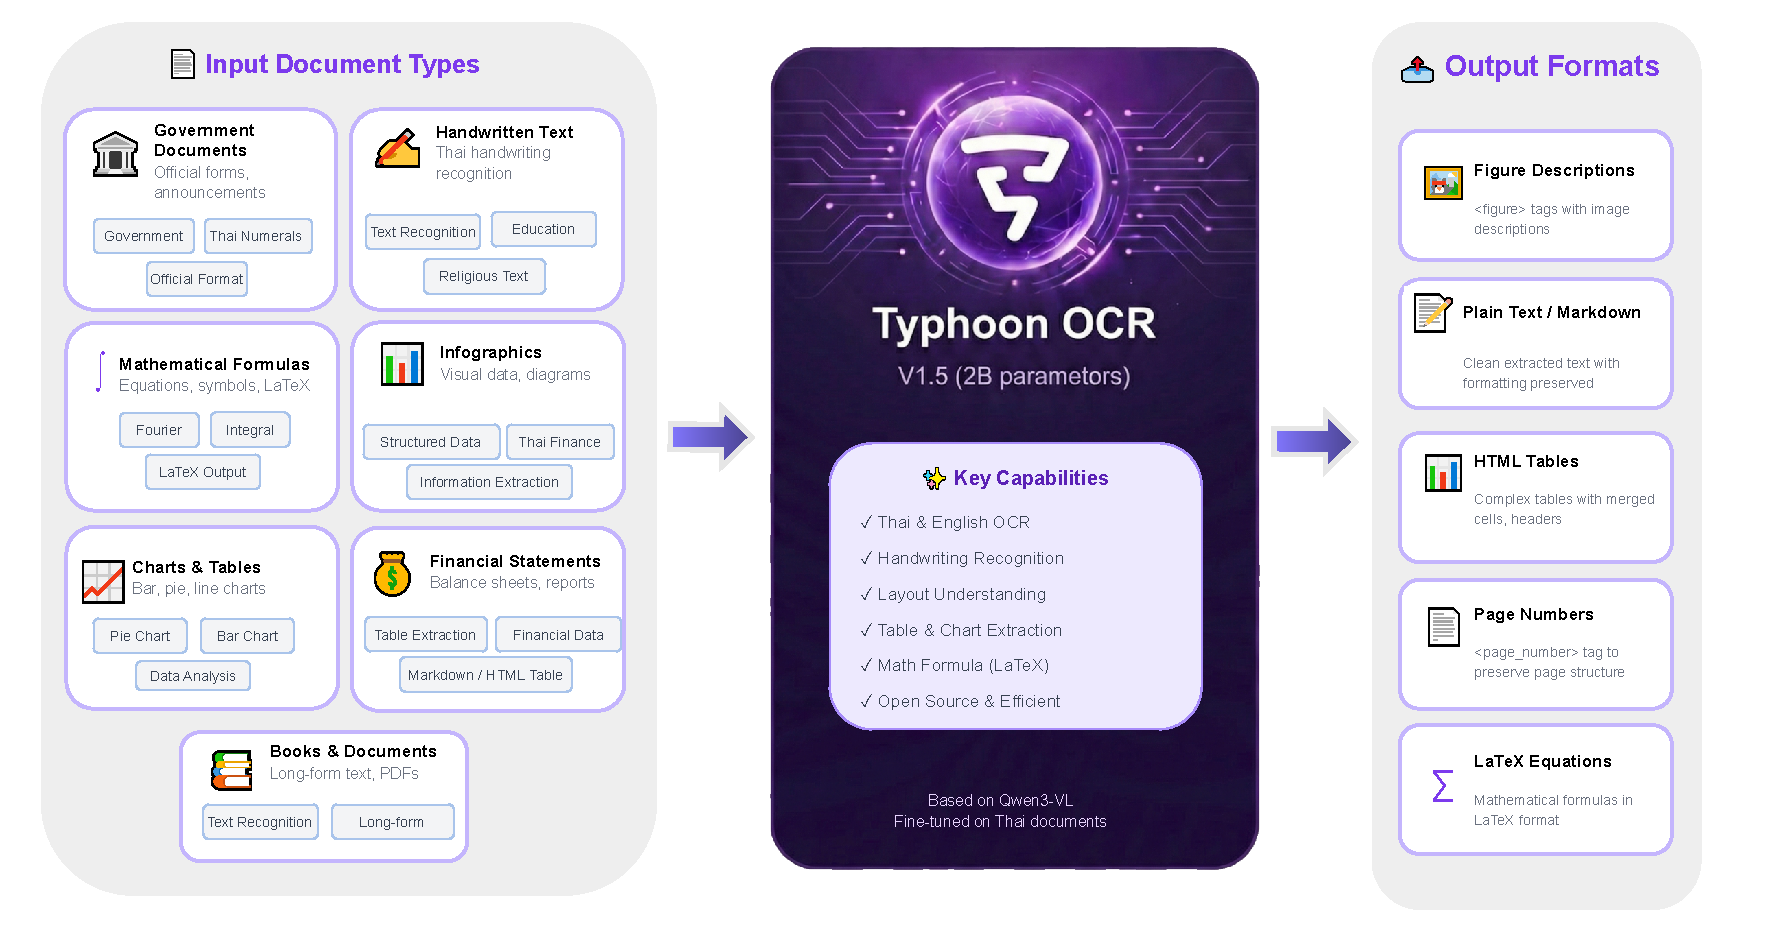
\includegraphics[width=0.95\textwidth]{picture/typhoon_ocr_overview.pdf}
    \caption{Overview of Typhoon OCR, illustrating supported input document types and the corresponding structured output representations.}
    \label{fig:overview_flow}
\end{figure}

Recent vision-language models (VLMs) are capable of various visual-language tasks from document understanding, integrating optical character recognition, layout analysis, to semantic modeling as a single model \citep{zhang2024visionlanguagemodelsvisiontasks}. While these models demonstrate strong performance on high-resource languages, their effectiveness degrades substantially in low-resource settings, particularly for languages with complex scripts and limited annotated data \citep{nonesung2025thaiocrbenchtaskdiversebenchmarkvisionlanguage}. Thai language is one such case, where linguistic properties and document diversity present persistent challenges for existing models.

% The Thai writing system exhibits characteristics that complicate document understanding. These include stacked diacritics, context-dependent vowel placement, and the absence of explicit word boundaries, all of which hinder reliable text segmentation and recognition \citep{4600388}. At the document level, Thai materials--such as administrative forms, financial records, receipts, and tabular reports--often contain dense and irregular layouts (see examples in \Cref{fig:overview_flow}). 

% The Thai writing system exhibits characteristics that complicate document understanding. These include stacked diacritics, context-dependent vowel placement, and the absence of explicit word boundaries, all of which hinder reliable text segmentation and recognition \citep{4600388}. At the document level, Thai materials--such as administrative forms, financial records, receipts, and tabular reports--often contain dense and irregular layouts, further increasing the difficulty of accurate extraction and structural reconstruction. Figure~\ref{fig:overview_flow} provides an overview of the document types supported by Typhoon OCR and the corresponding output representations. Accurate understanding therefore requires not only character-level transcription but also robust modeling of document layout and visual context. General-purpose VLMs, such as Qwen3 VL \citep{wei2025deepseekocrcontextsopticalcompression}, Gemma 3 \citep{gemmateam2025gemma3technicalreport}, InternVL 3.5 \citep{wang2025internvl35advancingopensourcemultimodal} predominantly trained on high-resource languages, frequently fail to capture these properties, resulting in elevated recognition errors, layout misinterpretation, and semantic inconsistencies.
The Thai writing system exhibits characteristics that complicate document understanding, including stacked diacritics, context-dependent vowel placement, and the absence of explicit word boundaries, all of which hinder reliable text segmentation and recognition \citep{4600388}. At the document level, Thai materials--such as administrative forms, financial records, receipts, and tabular reports--often contain dense and irregular layouts, further increasing the difficulty of accurate extraction and structural reconstruction.

\Cref{fig:overview_flow} provides an overview of the document types supported by Typhoon OCR and the corresponding output formats. Despite this range of document types and output requirements, general-purpose VLMs, such as Qwen3-VL \citep{wei2025deepseekocrcontextsopticalcompression}, Gemma 3 \citep{gemmateam2025gemma3technicalreport}, and InternVL 3.5 \citep{wang2025internvl35advancingopensourcemultimodal}, which are predominantly trained on high-resource languages, frequently fail to capture these properties, resulting in elevated recognition errors, layout misinterpretation, and semantic inconsistencies.

% A primary factor underlying these limitations is multimodal data scarcity \citep{}. In contrast to English or Chinese, Thai lacks large-scale datasets that align document images with structured textual and semantic annotations. 
A primary factor underlying these limitations is Thai data scarcity. The development of large language models (LLMs) for Thai has highlighted the broader challenge of limited high-quality Thai training data; recent Thai LLMs such as the Typhoon series are explicitly designed and evaluated on Thai language datasets to improve Thai language processing \citep{typhoon2}. This issue is more prevalent in multimodal data. In contrast to English or Chinese, Thai lacks large-scale datasets that align document images with structured textual and semantic annotations, limiting the adaptability of existing models.
% Consequently, pretrained VLMs have limited exposure to Thai-specific visual and linguistic patterns, restricting their ability to generalize across domains such as public administration, finance, and education. This imbalance is further reflected in the ecosystem of available tools: proprietary models often achieve stronger empirical performance but remain opaque and inaccessible, whereas open alternatives offer higher transparency and flexibility but underperform on Thai document benchmarks \hl{see comments}.
Consequently, many of existing VLMs have limited exposure to Thai-specific visual and linguistic patterns, restricting their ability to generalize across domains such as public administration, finance, and education. This imbalance is reflected in our evaluations (Tables~\ref{tab:typhoon_eval},~\ref{tab:bleu_by_task}–\ref{tab:lev_by_task}), where proprietary models such as GPT and Gemini achieve competitive performance on some categories but are generally outperformed by Typhoon OCR on structured Thai document extraction tasks.

% These challenges motivate the development of a document understanding system explicitly adapted to Thai. Prior research in low-resource OCR and natural language processing suggests that fine-tuning large pretrained models with language- and domain-specific supervision can yield substantial gains without requiring training from scratch \citep{}. In the context of VLMs, this approach potentially enables the reuse of general visual-linguistic representations while addressing language-specific deficiencies through targeted data curation and adaptation. Empirical studies also indicate that zero-shot multilingual models perform poorly on Thai document tasks, reinforcing the need for dedicated fine-tuning \citep{}.

These challenges motivate the development of a document understanding model explicitly adapted to Thai. Prior research in low-resource optical character recognition (OCR) and multilingual natural language processing suggests that fine-tuning large pretrained models with language- and domain-specific supervision can yield substantial gains without requiring training from scratch. For example, adapting multilingual vision–language transformers to low-resource OCR tasks has been shown to improve recognition performance in non-Latin scripts \citep{cheema2024adapting}, and synthetic data augmentation and fine-tuning have been used to improve OCR performance across diverse low-resource languages \citep{ignat-etal-2022-ocr}. Similarly, transfer learning and fine-tuning of pretrained multilingual models have been effective in low-resource machine translation settings \citep{dalal-etal-2024-ai}, illustrating the broader utility of model adaptation in low-resource linguistic domains.

In this work, we present \textbf{Typhoon OCR}, an open VLM for end-to-end Thai and English document understanding. The model is capable of various visual-language capabilities, including text extraction, layout reconstruction, and document-level semantic modeling. Typhoon OCR is obtained by fine-tuning an open VLM backbone using a task-aligned training corpus constructed from curated real-world documents and synthetic data. By explicitly modeling document structure alongside textual content, our model has capabilities beyond traditional OCR pipelines focused primarily on transcription. Our contributions are as follows:
\begin{itemize}[leftmargin=*]
\setlength\itemsep{-0.1em}
    \item We introduce Typhoon OCR, an open VLM tailored to Thai document extraction.
    \item We propose a data curation and synthesis pipeline that mitigates multimodal data scarcity for Thai.
    \item We comprehensively evaluate our models against the baselines, demonstrating improvements over existing open baselines and competitive performance relative to proprietary models on Thai document benchmarks.
    \item Our models and associated resources are released under permissive licenses to support reproducible research and practical deployment.
\end{itemize}


\section{Typhoon OCR}
%
Typhoon OCR is an open VLM for end-to-end document extraction in Thai and English, including text recognition and layout-aware content reconstruction. It targets real-world documents with complex and heterogeneous layouts, where existing OCR pipelines and general-purpose VLMs perform poorly in low-resource settings.

The model is trained by fine-tuning a vision-language backbone on a task-aligned corpus combining curated real documents and synthetic data. Experiments show that Typhoon OCR substantially outperforms existing open-source methods and achieves competitive performance relative to proprietary models on Thai document benchmarks.


\subsection{Data}
\subsubsection{Dataset Creation Pipeline}
\begin{table}[h]
\centering
\begin{tabular}{@{}p{4cm}p{5.5cm}p{5.5cm}@{}}
\toprule
\textbf{Feature} & \textbf{Default Mode} & \textbf{Structure Mode} \\
\midrule
\textbf{Target Documents} &
Loosely structured or unstructured documents, such as receipts, menus, tickets, infographics, and handwritten notes. &
Highly structured documents with complex layouts, including financial reports, academic papers, government forms, and books. \\
\midrule
\textbf{Layout Modeling} &
Lightweight layout preservation with an emphasis on content continuity and readability. &
Explicit structural parsing with detailed reconstruction of hierarchical and semantic regions. \\
\midrule
\textbf{Output Representation} &
Only \texttt{Markdown} with minimal layout annotations. &
\texttt{Markdown} for narrative text, \texttt{HTML} for complex tables and structured layouts, and \texttt{<figure>} tags for visual elements. \\
\bottomrule
\end{tabular}
\caption{Comparison of supervision modes used in Typhoon OCR.}
\label{tab:modes-comparison}
\end{table}
% To support heterogeneous document types, we construct a training corpus that enables the model to operate in two complementary modes, which differ in output representation and layout fidelity. These modes are: \emph{Default Mode}, targeting unstructured documents, and \emph{Structure Mode}, targeting structured documents with complex layouts. Details are provided in \Cref{tab:modes-comparison}. The separation enables the model to learn both flexible content extraction and precise structural reconstruction, depending on document characteristics.

To support different types of documents, we construct a training corpus that allows the model to operate in two modes: \emph{Default Mode} and \emph{Structure Mode}. These modes differ in how much layout information is preserved in the output. A single supervision format is not suitable for both loosely structured documents (such as receipts or handwritten notes) and highly structured documents (such as financial reports or government forms). Using one format for all cases would either add unnecessary complexity to simple documents or fail to capture important layout details in complex ones.

We therefore adopt two modes as a simple and practical division based on document structure: documents with little or weak layout structure, and documents with clear and complex layout organization. This separation covers most document types in our dataset without introducing excessive design complexity.

This design also follows the availability of training data. Default Mode reuses general document annotations from the Typhoon2 Vision training corpus~\citep{typhoon2}. Structure Mode, in contrast, is newly created using the dataset construction pipeline shown in \Cref{fig:dataset_flow}, which produces structure-aware annotations for complex documents. In practice, users choose the mode based on the document type, as summarized in \Cref{tab:modes-comparison}.





% \begin{table}[h]
% \centering
% \begin{tabular}{@{}p{4cm}p{5.5cm}p{5.5cm}@{}}
% \toprule
% \textbf{Feature} & \textbf{Default Mode} & \textbf{Structure Mode} \\
% \midrule
% \textbf{Target Documents} &
% Loosely structured or unstructured documents, such as receipts, menus, tickets, infographics, and handwritten notes. &
% Highly structured documents with complex layouts, including financial reports, academic papers, government forms, and books. \\
% \midrule
% \textbf{Layout Modeling} &
% Lightweight layout preservation with an emphasis on content continuity and readability. &
% Explicit structural parsing with detailed reconstruction of hierarchical and semantic regions. \\
% \midrule
% \textbf{Output Representation} &
% Only \texttt{Markdown} with minimal layout annotations. &
% \texttt{Markdown} for narrative text, \texttt{HTML} for complex tables and structured layouts, and \texttt{<figure>} tags for visual elements. \\
% \bottomrule
% \end{tabular}
% \caption{Comparison of supervision modes used in Typhoon OCR.}
% \label{tab:modes-comparison}
% \end{table}

\begin{figure}[htbp]
    \centering
    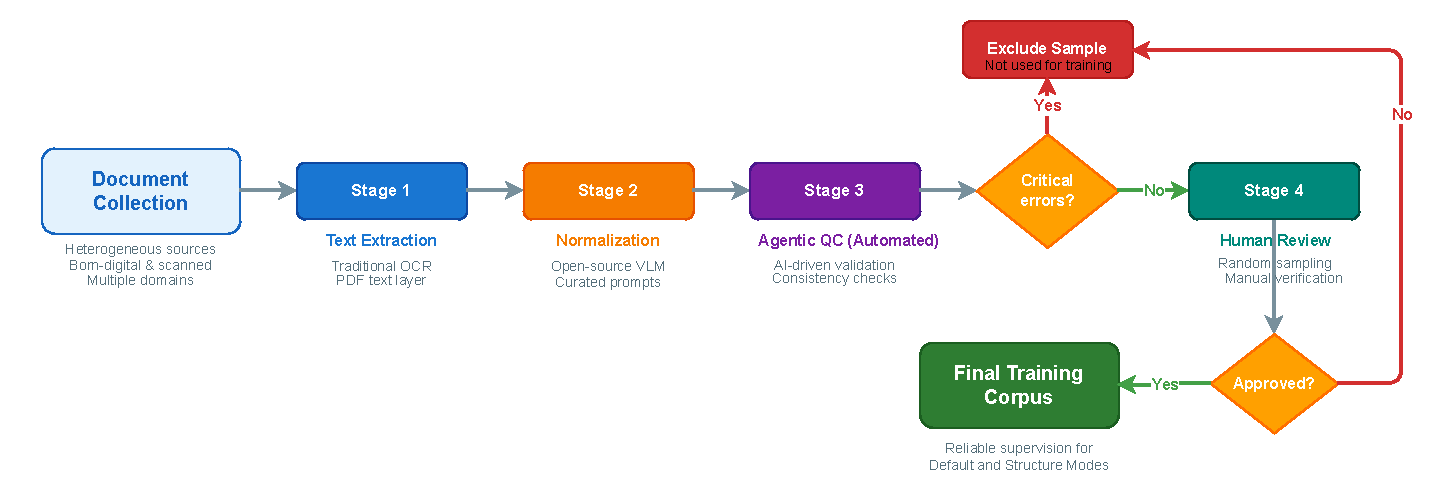
\includegraphics[width=\linewidth]{picture/document_collection_pipeline.pdf}
    \caption{Overview of the multi-stage dataset construction pipeline used to generate training data for Typhoon OCR under Structure Mode.}
    \label{fig:dataset_flow}
\end{figure}


As shown in \Cref{fig:dataset_flow}, the training data are collected from diverse sources, including digital-native documents and scanned materials spanning multiple domains. Rather than applying a single processing strategy, we use a multi-stage pipeline that incrementally refines annotations while balancing scalability and supervision quality. These stages are:

\paragraph{Stage 1} Textual content is extracted using conventional OCR systems and, where available, document text-layer parsing. This stage focuses on reliable character- and word-level transcription, particularly for clean digital documents and high-resolution scans, and provides a stable low-level supervision signal.

\paragraph{Stage 2} The extracted text is reorganized using open-source VLMs guided by structured prompts. This step transforms raw OCR outputs into coherent document representations by incorporating layout-aware formatting, section grouping, and basic semantic organization.

\paragraph{Stage 3} Automated quality control is applied through agent-based consistency checks. These checks detect common failure modes, including structural inconsistencies, missing or duplicated content, incorrect ordering, and misalignment between visual input and generated annotations.

\paragraph{Stage 4} A subset of samples is selected for human verification. Annotators assess annotation fidelity with respect to the source documents, and samples exhibiting substantial or irrecoverable errors are removed from the corpus.

This multi-stage pipeline enables scalable dataset construction while mitigating noise from automated annotation. As a result, the final corpus provides consistent, high-quality supervision for fine-tuning Typhoon OCR under both modes.




% \subsubsection{Dataset statistic}
% Figure~\ref{fig:dataset_dis} shows the distribution of the training dataset. We collect and curate data from publicly available sources in both Thai and English, including infographics, government forms, financial reports, and more.


% To generate high-quality annotations, we use Qwen2.5-VL-70B as a labeling assistant. We further enhance data quality through random manual checks by human annotators to ensure high fidelity and consistency. For detail implements, please refer to Typhoon 2 technical report ~\citep{pipatanakul2024typhoon2familyopen}.


% \begin{figure}[htbp]
%     \centering
%     \begin{subfigure}{0.49\textwidth}
%         \centering
%         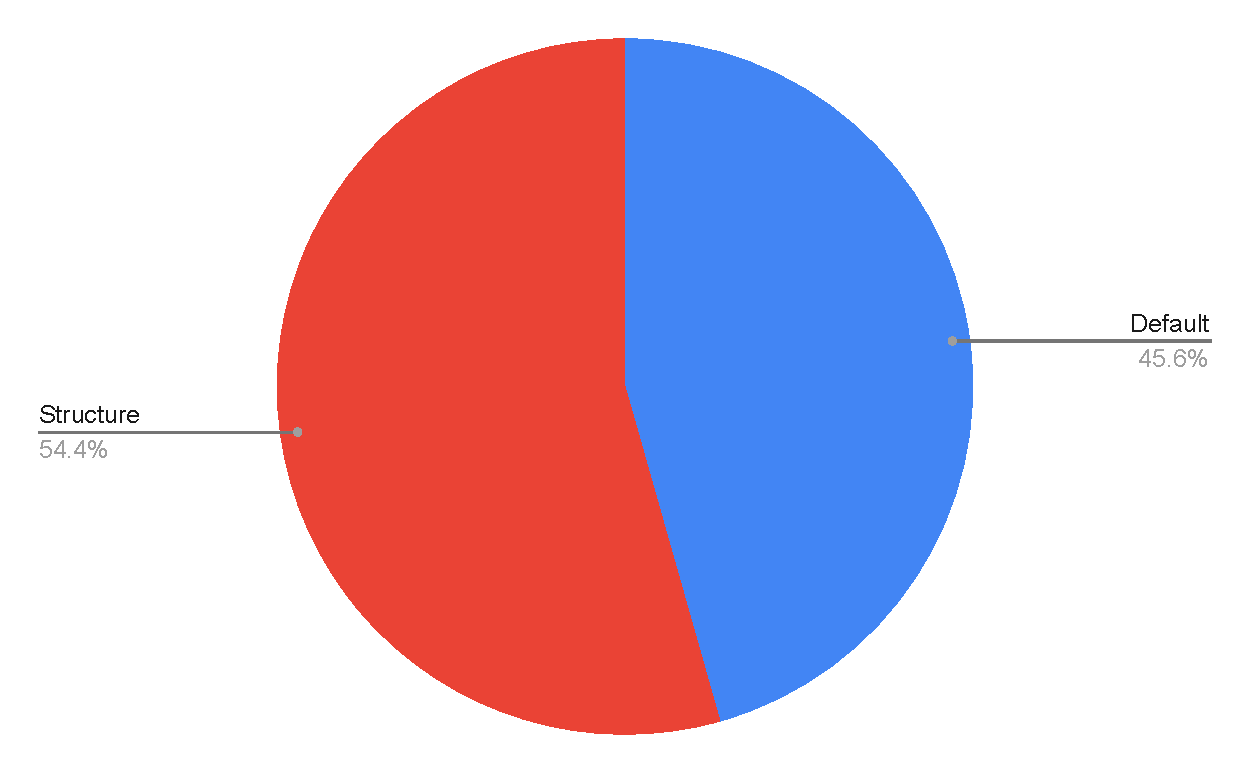
\includegraphics[width=\textwidth]{picture/chart1.pdf}
%         \caption{Training dataset distribution}
%         \label{fig:dataset_dis}
%     \end{subfigure}
%     \hfill
%     \begin{subfigure}{0.49\textwidth}
%         \centering
%         \includegraphics[width=\textwidth]{picture/info.pdf}
%         \caption{Training data by source}
%         \label{fig:dataset_by}
%     \end{subfigure}
%     \caption{Overview of the datasets used for fine-tuning Typhoon OCR}
% \end{figure}

% Figure~\ref{fig:dataset_by} illustrates the distribution of our training dataset by sources, which comprises diverse document types in both Thai and English. The dataset is composed of the following major categories:

% \begin{itemize}
%     \item \textbf{General Infographics (45.6\%):} This is the largest category, consisting of a wide range of infographic-style content from web and public data sources.
%     \item \textbf{Cosyn (8.3\%):} Sourced from the CoSyn-400K dataset\footnote{\url{https://huggingface.co/datasets/allenai/CoSyn-400K}}, which contains synthetic documents with structured layouts.
%     \item \textbf{Thai Financial Reports (7.2\%):} Includes financial statements and investor documents from Thai organizations.
%     \item \textbf{Thai Books (5.6\%)} Includes Thai books.
%     \item \textbf{Handwriting\_iapp (5.5\%):} The latter is derived from the IAPP Thai handwriting dataset\footnote{\url{https://huggingface.co/datasets/iapp/thai_handwriting_dataset}}, comprising handwritten forms and letters. we sample from this dataset because some labeling is wrong.
%     \item \textbf{Olm Documents (3.1\% and Olm Books (3.1\%))} Taken from the OlmOCR-mix-0225 dataset\footnote{\url{https://huggingface.co/datasets/allenai/olmOCR-mix-0225}}, representing scanned documents and books.
%     \item \textbf{Thai Innovesting Reports (2.9\%), Financial Infographics (2.9\%), and Bill \& Invoice (2.9\%):} Various structured and semi-structured financial and transactional documents.
%     \item \textbf{Others (13.0\%)} Includes various long-tail document types such as government forms, certificates, academic papers, and miscellaneous scans.

% \end{itemize}
% \subsection{Dataset Statistics}

% Figure~\ref{fig:dataset_dis} presents the overall distribution of the training dataset used for fine-tuning Typhoon OCR. The corpus is collected and curated from publicly available sources in both Thai and English, covering a wide range of document types, including infographics, government forms, financial reports, books, and handwritten materials.

% \begin{figure}[htbp]
%     \centering
%     \begin{subfigure}{0.49\textwidth}
%         \centering
%         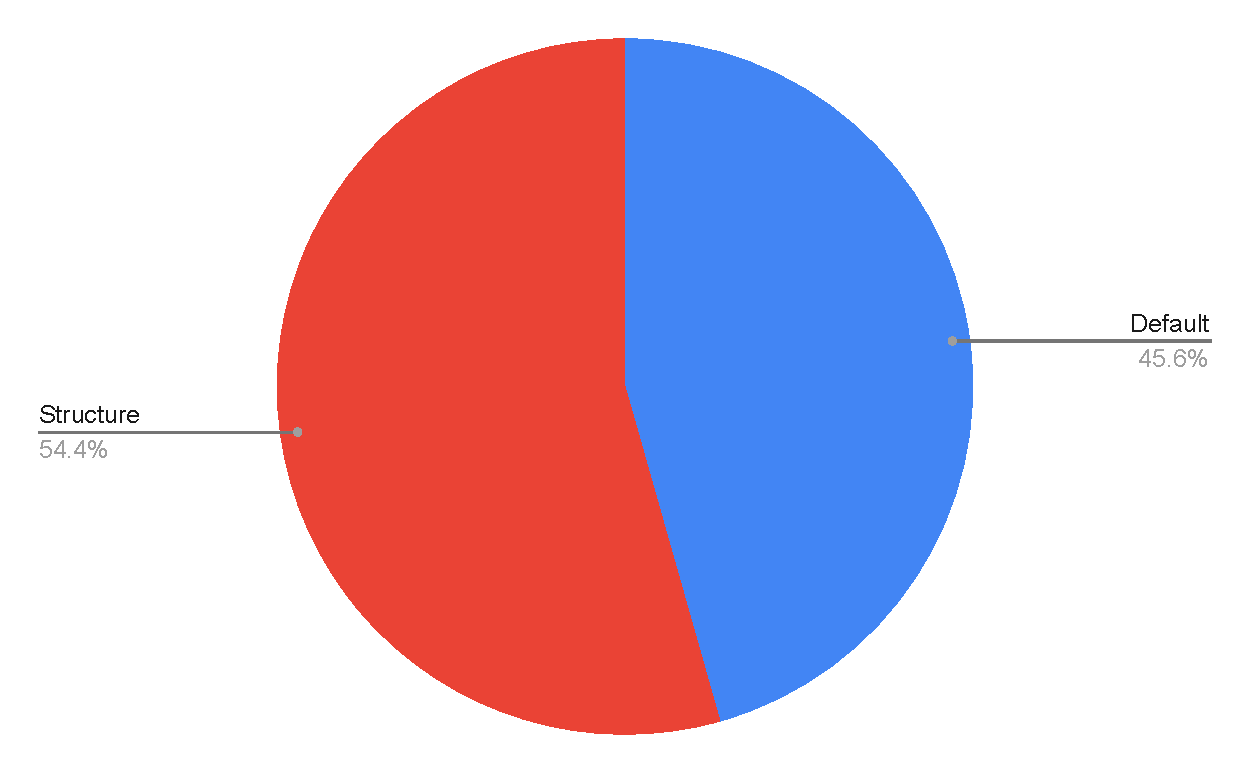
\includegraphics[width=\textwidth]{picture/chart1.pdf}
%         \caption{Distribution of the training dataset}
%         \label{fig:dataset_dis}
%     \end{subfigure}
%     \hfill
%     \begin{subfigure}{0.49\textwidth}
%         \centering
%         \includegraphics[width=\textwidth]{picture/info.pdf}
%         \caption{Training data by source}
%         \label{fig:dataset_by}
%     \end{subfigure}
%     \caption{Overview of the datasets used for fine-tuning Typhoon OCR}
% \end{figure}

% Figure~\ref{fig:dataset_by} shows the distribution of the training data by source. The dataset comprises a diverse mixture of document types across both languages, reflecting realistic document variability. The major data categories are summarized as follows:

% \begin{itemize}
%     \item \textbf{General Infographics (45.6\%):} The largest category, consisting of a broad range of infographic-style documents collected from web and public data sources.
    
%     \item \textbf{CoSyn (8.3\%):} Derived from the CoSyn-400K dataset\footnote{\url{https://huggingface.co/datasets/allenai/CoSyn-400K}}, which provides synthetically generated documents with structured layouts.
    
%     \item \textbf{Thai Financial Reports (7.2\%):} Financial statements, investor presentations, and related documents published by Thai organizations.
    
%     \item \textbf{Thai Books (5.6\%):} Digitized Thai books encompassing a range of genres and formatting styles.
    
%     \item \textbf{Handwriting\_IAPP (5.5\%):} Sampled from the IAPP Thai handwriting dataset\footnote{\url{https://huggingface.co/datasets/iapp/thai_handwriting_dataset}}, which includes handwritten forms and letters. Subsampling is applied to mitigate known labeling inconsistencies.
    
%     \item \textbf{OLMOCR Documents (3.1\%) and OLMOCR Books (3.1\%):} Collected from the OLMOCR-mix-0225 dataset\footnote{\url{https://huggingface.co/datasets/allenai/olmOCR-mix-0225}}, representing scanned documents and book pages.
    
%     \item \textbf{Thai InnovestX Reports (2.9\%), Financial Infographics (2.9\%), and Bills \& Invoices (2.9\%):} A collection of structured and semi-structured financial and transactional documents.
    
%     \item \textbf{Others (13.0\%):} A long-tail category including government forms, certificates, academic papers, and miscellaneous scanned documents.
% \end{itemize}

\subsubsection{Dataset Statistics}

\Cref{fig:dataset_dis} summarizes the composition of the training corpus used to fine-tune Typhoon OCR. The dataset is curated from publicly available sources in both Thai and English and spans a wide range of document types, including infographics, government forms, financial reports, books, and handwritten materials. This diversity is intended to reflect realistic variation in document layout, visual quality, and linguistic content encountered in practical document understanding tasks.

\begin{figure}[htbp]
    \centering
    \begin{subfigure}{0.45\textwidth}
        \centering
        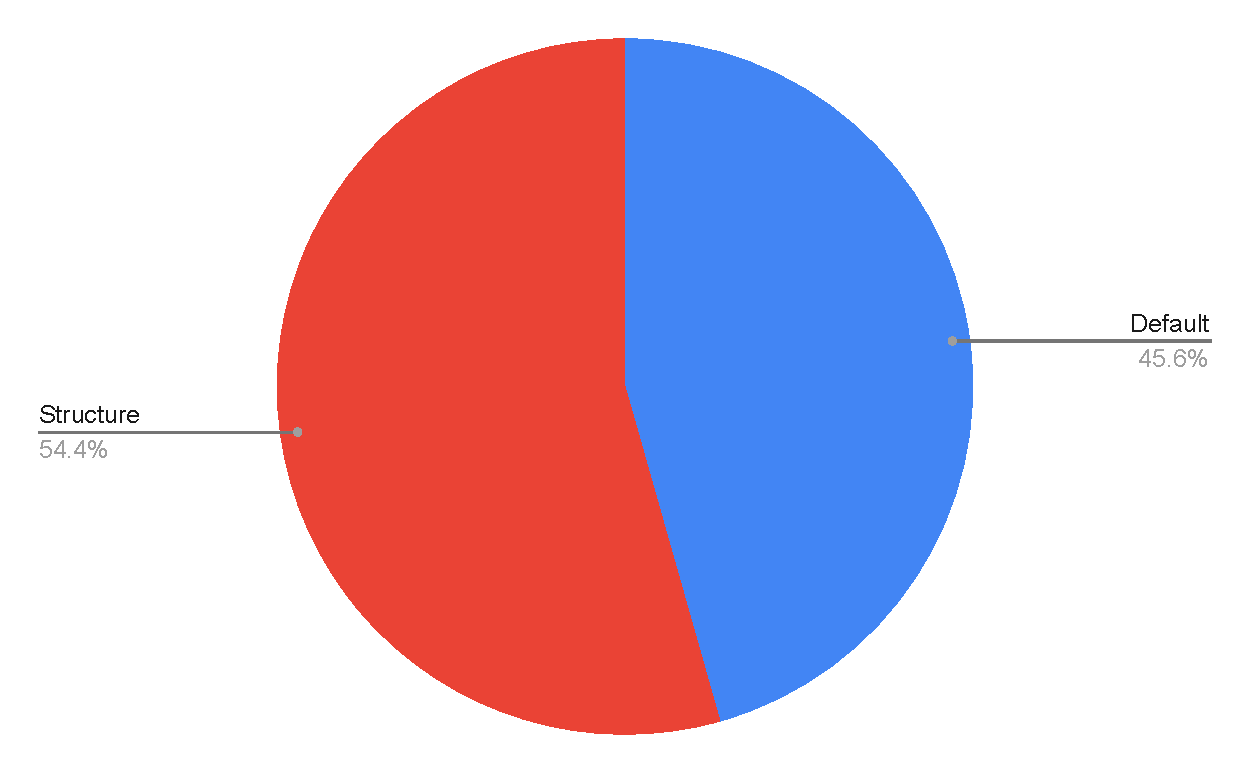
\includegraphics[width=\textwidth]{picture/chart1.pdf}
        \caption{Distribution of training samples across modes}
        \label{fig:dataset_dis}
    \end{subfigure}
    \hfill
    \begin{subfigure}{0.5\textwidth}
        \centering
        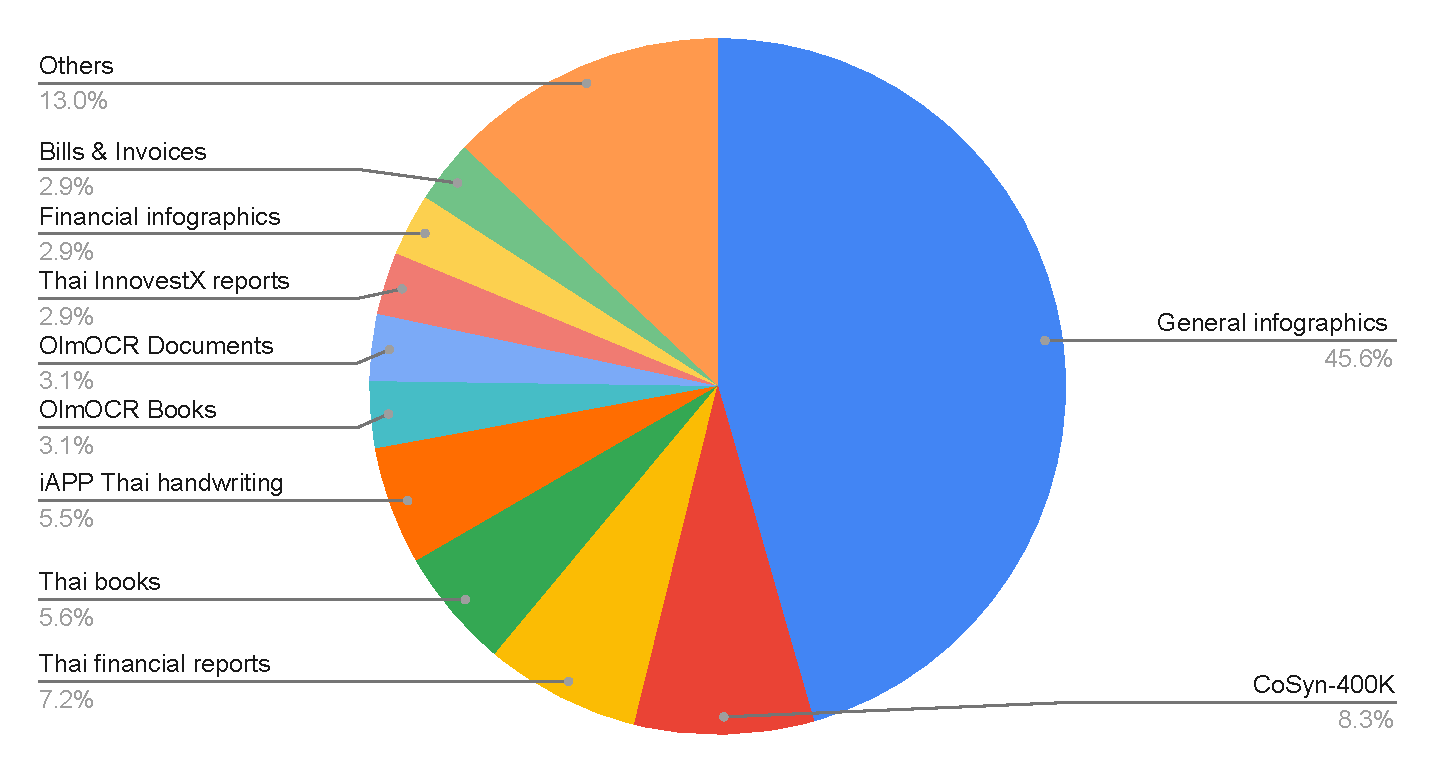
\includegraphics[width=\textwidth]{picture/info2.pdf}
        \caption{Distribution of training samples by data source}
        \label{fig:dataset_by}
    \end{subfigure}
    \caption{Composition of the training corpus used for Typhoon OCR. Figure~\ref{fig:dataset_dis} shows the allocation of samples between Default Mode and Structure Mode supervision, while Figure~\ref{fig:dataset_by} presents the relative contributions of different data sources.}
\end{figure}

% , with Structure Mode data ratio slightly higher than Default Mode data.

As shown in \Cref{fig:dataset_by}, the corpus consists of a heterogeneous mixture of document sources across both languages. General infographic-style documents constitute the largest portion of the dataset (45.6\%), providing broad coverage of diverse layouts and visual styles. Structured synthetic documents from the CoSyn-400K dataset\footnote{\url{https://huggingface.co/datasets/allenai/CoSyn-400K}} \citep{yang2025scaling} account for 8.3\% of the corpus and provide controlled layout variations that facilitate learning of document structure.

Domain-specific Thai documents form a substantial component of the dataset. These include financial reports published by Thai SET organizations (7.2\%), digitized Thai books spanning multiple genres and formatting conventions (5.6\%), and handwritten materials sampled from the iAPP Thai handwriting dataset\footnote{\url{https://huggingface.co/datasets/iapp/thai_handwriting_dataset}} (5.5\%). For the handwriting data, subsampling is applied to mitigate the impact of known labeling inconsistencies.

Additional scanned documents and book pages are drawn from the olmOCR-mix-0225 collection\footnote{\url{https://huggingface.co/datasets/allenai/olmOCR-mix-0225}}, contributing a combined 6.2\% of the corpus. The remaining portion of the dataset comprises Thai InnovestX reports, financial infographics, and bills and invoices (8.7\%), alongside a long-tail category (13.0\%) that includes government forms, certificates, academic papers, and other miscellaneous scanned documents. In total, the training corpus contains 77,029 document samples.


% \subsection{Training Settings}

% We perform supervised fine-tuning (SFT) on the Qwen2.5-VL model family, using the 3B and 7B parameter variants with full-parameter optimization. The training pipeline is adapted from the open-source \texttt{olmOCR} repository\footnote{\url{https://github.com/allenai/olmocr}}, with modifications to support multilingual document parsing and extended sequence lengths.

% During preprocessing, input images are resized to a fixed width of 1{,}800 pixels to balance visual resolution and computational efficiency. The anchor text length is set to 8{,}000 tokens, and the total sequence length is capped at 17{,}000 tokens to accommodate long-form documents and complex layouts.

% Training is conducted on four GPUs, each equipped with 80\,GB of memory. Models are trained for three epochs, and the final checkpoint is selected based on performance on a held-out evaluation set. This configuration enables stable optimization while preserving the model's capacity to capture long-range dependencies and detailed layout information.

% \subsection{Evaluation and Results}

% \subsubsection{Evaluation Methodology}
% To assess the performance of Typhoon OCR, we adopt standard evaluation metrics commonly used in optical character recognition (OCR) and natural language generation (NLG) tasks:

% \begin{itemize}
%     \item \textbf{BLEU:} Measures n-gram precision between the predicted and reference texts. Higher scores indicate better lexical overlap.
    
%     \item \textbf{ROUGE-L:} Evaluates the longest common subsequence between generated and reference sequences, capturing both structural and sequential similarities.
    
%     \item \textbf{Levenshtein Distance:} Computes the character-level edit distance. Lower values indicate greater textual accuracy.
% \end{itemize}

% These metrics allow us to evaluate both the textual fidelity and structural integrity of Typhoon OCR's outputs across a diverse range of document types.

% \subsection{Experimental Setup}
% We evaluate Typhoon OCR in two input settings to understand its robustness across different formats:

% \begin{itemize}
%     \item \textbf{PDF with Metadata:} The model is provided with native document metadata, including text layers and layout annotations.
    
%     \item \textbf{Image-Only Input:} The model receives rasterized inputs (e.g., \texttt{.jpeg}, \texttt{.png}, or scanned PDFs) without access to metadata.
% \end{itemize}

% We compare Typhoon OCR against two state-of-the-art vision-language baselines:

% \begin{itemize}
%     \item \textbf{GPT-4o} (released 2024-11-20)
%     \item \textbf{Gemini 2.5 Flash Preview} (released 2025-04-17)
% \end{itemize}

% These systems represent the latest advancements in commercial and research-grade vision-language OCR technologies.

% \subsection{Evaluation and Results}

% \subsubsection{Evaluation Methodology}

% To assess the performance of Typhoon OCR, we adopt standard evaluation metrics commonly used in optical character recognition (OCR) and natural language generation (NLG). These metrics capture complementary aspects of output quality at both the lexical and structural levels:

% \begin{itemize}
%     \item \textbf{BLEU}~\citep{papineni-etal-2002-bleu}: Measures $n$-gram precision between predicted and reference texts, reflecting lexical overlap and transcription accuracy. Higher scores indicate better performance.
    
%     \item \textbf{ROUGE-L}~\citep{lin-2004-rouge}: Computes the longest common subsequence between generated and reference sequences, capturing both structural similarity and sequence coherence.
    
%     \item \textbf{Levenshtein Distance}~\citep{haldar2011levenshteindistancetechniquedictionary}: Measures character-level edit distance. Lower values indicate fewer transcription errors and higher textual fidelity.
% \end{itemize}

% Together, these metrics enable a comprehensive evaluation of Typhoon OCR's ability to preserve textual content, document structure, and sequential consistency across a diverse range of document types and layouts.

% \subsubsection{Experimental Setup}

% We evaluate Typhoon OCR under two input conditions to examine its robustness across different document representations:

% \begin{itemize}
%     \item \textbf{PDF with Metadata:} The model is provided with native PDF metadata, including text layers, bounding boxes, and layout annotations, when available.
    
%     \item \textbf{Image-Only Input:} The model receives rasterized document images (e.g., \texttt{.jpeg}, \texttt{.png}, or scanned PDFs) without access to structural metadata.
% \end{itemize}

% This experimental design allows us to analyze the model's ability to leverage explicit layout information when present, as well as its capacity to infer structure directly from visual input when metadata is unavailable.
\subsection{Experimental Setup}

\subsubsection{Training}

Typhoon OCR is trained using full-parameter supervised fine-tuning (SFT) on the Qwen2.5-VL model family \citep{bai2025qwen25vltechnicalreport}, covering both the 3B and 7B parameter variants. The training pipeline is based on the open-source \texttt{olmOCR} framework\footnote{\url{https://github.com/allenai/olmocr}} \citep{poznanski2025olmocrunlockingtrillionstokens}, with extensions to support multilingual document understanding and long-context modeling. The models are trained on 4$\times$H100 GPUs for three epochs, and the final checkpoint is selected based on performance on a held-out validation set.

Input document images are resized to a fixed width of 1,800 pixels, providing a trade-off between visual fidelity and computational efficiency. The anchor text length is set to 8,000 tokens to balance layout coverage and memory constraints, and the maximum sequence length is limited to 17,000 tokens, allowing the model to process long-form documents and dense layouts without truncation.

% \subsubsection{Evaluation Methodology}

% We evaluate Typhoon OCR using standard metrics from optical character recognition and natural language generation that capture complementary aspects of output quality. Lexical accuracy is assessed using BLEU~\citep{papineni-etal-2002-bleu}, which measures $n$-gram overlap between predicted and reference texts. Structural and sequential similarity is measured using ROUGE-L~\citep{lin-2004-rouge}, based on the longest common subsequence. Although originally designed for NLG, these metrics correlate well with document reconstruction fidelity in structured outputs. Character-level transcription fidelity is quantified using Levenshtein distance~\citep{haldar2011levenshteindistancetechniquedictionary}, where lower values indicate fewer edit operations.
\subsubsection{Evaluation}\label{sec:v1_eval}

\paragraph{Metrics}
We evaluate Typhoon OCR using standard metrics from OCR and natural language generation (NLG) that capture complementary aspects of output quality. Lexical accuracy is assessed using \textbf{BLEU} \citep{papineni-etal-2002-bleu}, which measures $n$-gram overlap between predicted and reference texts. Structural and sequential similarity is measured using \textbf{ROUGE-L} \citep{lin-2004-rouge}, based on the longest common subsequence. Although originally developed for NLG, these metrics correlate well with document extraction in structured outputs. Character-level transcription fidelity is quantified using \textbf{Levenshtein distance} \citep{haldar2011levenshteindistancetechniquedictionary}, where lower values indicate fewer edit operations.

\paragraph{Benchmark}
Evaluation is conducted on an in-house Thai document corpus designed to reflect real-world document variability in both layout and content. The corpus comprises three categories: Thai financial reports, which include complex tables, charts, and multilingual content; Thai government forms, characterized by dense layouts, domain-specific terminology, and handwritten annotations; and Thai books, consisting of long-form text interleaved with figures, diagrams, and other visual elements.

\paragraph{Protocol}

Evaluation is conducted under two input conditions to examine robustness across document representations. In the \emph{PDF with metadata} setting, the model is provided with native PDF information, including text layers and layout annotations, when available. In the \emph{image-only} setting, the model receives rasterized document images without access to structural metadata.

This setup isolates the contribution of explicit layout information and allows analysis of the model's ability to infer document structure directly from visual input.

% We compare Typhoon OCR against two state-of-the-art vision--language baselines representing leading commercial document understanding systems:

% \begin{itemize}
%     \item \textbf{GPT-4o} (release date: 2024-11-20)~\citep{openai2024gpt4technicalreport}
%     \item \textbf{Gemini 2.5 Flash Preview} (release date: 2025-04-17)~\citep{geminiteam2025geminifamilyhighlycapable}
% \end{itemize}

% All models are evaluated on the same held-out test set using identical prompts and output formats to ensure a fair and controlled comparison.


% \subsubsection{Evaluation Datasets}
% Evaluation was performed using an in-house Thai document corpus designed to capture real-world layout complexity and domain diversity. The dataset consists of the following categories:

% \begin{itemize}
%     \item \textbf{Thai Financial Reports:} Structured documents containing tables, charts, and mixed multilingual content.
    
%     \item \textbf{Thai Government Forms:} Forms with dense layouts, handwritten annotations, and domain-specific terminology.
    
%     \item \textbf{Thai Books:} Long-form textual documents interleaved with various visual elements, including diagrams, illustrations, and embedded figures.
% \end{itemize}

% \begin{table}[htbp]
%     \centering
%     \begin{tabular}{lccc}
%         \toprule
%         \textbf{Model} & \textbf{BLEU}\textcolor{teal}{$\uparrow$} & \textbf{ROUGE-L}\textcolor{teal}{$\uparrow$} & \textbf{Levenshtein}\textcolor{red}{$\downarrow$} \\
%         \midrule
%         \rowcolor{Gray}
%         \multicolumn{4}{l}{\textbf{Thai Financial Reports}} \\
%         GPT-4o (2024-11-20) & 0.25 & 0.51 & 0.56 \\
%         Gemini 2.5 Flash (2025-04-17) & 0.52 & 0.70 & 0.35 \\
%         Typhoon OCR 3B (PDF) & 0.90 & 0.93 & 0.08 \\
%         Typhoon OCR 3B (Image) & 0.90 & 0.93 & \textbf{0.07} \\
%         Typhoon OCR 7B (PDF) & \textbf{0.91} & \textbf{0.94} & \textbf{0.07} \\
%         Typhoon OCR 7B (Image) & \textbf{0.91} & \textbf{0.94} & 0.08 \\
%         \rowcolor{Gray}
%         \multicolumn{4}{l}{\textbf{Thai Government Forms}} \\
%         GPT-4o (2024-11-20) & 0.25 & 0.45 & 0.57 \\
%         Gemini 2.5 Flash (2025-04-17) & 0.74 & 0.87 & 0.15 \\ 
%         Typhoon OCR 3B (PDF)& 0.92 & \textbf{0.96} & 0.05 \\
%         Typhoon OCR 3B (Image) & \textbf{0.93} & \textbf{0.96} & \textbf{0.04} \\
%         Typhoon OCR 7B (PDF)& 0.89 & 0.94 & 0.08 \\
%         Typhoon OCR 7B (Image) & 0.89 & 0.94 & 0.07 \\
%         \rowcolor{Gray}
%         \multicolumn{4}{l}{\textbf{Thai Books}} \\
         
%         GPT-4o (2024-11-20) & 0.34 & 0.49 & 0.59 \\
%         Gemini 2.5 Flash (2025-04-17) & 0.47 & 0.59 & 0.47 \\
%         Typhoon OCR 3B (PDF)& 0.63 & 0.71 & 0.32 \\
%         Typhoon OCR 3B (Image) & \textbf{0.64} & 0.71 & 0.32 \\
%         Typhoon OCR 7B (PDF)& 0.63 & 0.71 & \textbf{0.31} \\
%         Typhoon OCR 7B (Image) & \textbf{0.64} & \textbf{0.72} & \textbf{0.31} \\
%         \bottomrule 
%     \end{tabular}
%     \caption{Performance comparison of Typhoon OCR on structure mode with state-of-the-art vision-language models on Thai document parsing. Higher BLEU and ROUGE-L and lower Levenshtein indicate better performance.}
%     \label{tab:typhoon_eval}
% \end{table}
% \subsection{Results and Discussion}

% \textbf{Results.}  
% Table~\ref{tab:typhoon_eval} reports the evaluation results for Typhoon OCR (3B and 7B) compared with GPT-4o and Gemini~2.5~Flash on Thai document understanding tasks. Across most document categories, Typhoon OCR achieves higher performance, particularly on documents with complex layouts and mixed Thai--English content, such as financial reports and government forms. These gains are largely attributable to the integration of vision--language modeling with explicit document structure cues derived from PDF metadata.

% Performance is comparatively lower on the Thai Books subset, which presents additional challenges due to the frequent presence of heterogeneous visual elements, including illustrations, charts, and non-standard figures. Such elements increase layout complexity and introduce ambiguity in figure representation, leading to less accurate generation of \texttt{<figure>} tags. This result indicates limitations in the current visual understanding and figure interpretation components and highlights an area for future improvement.

% The performance gap between PDF-based inputs and image-only inputs is relatively small for Typhoon OCR, suggesting effective alignment between visual and textual representations. In addition, the 3B model variant achieves competitive results, particularly on government forms, indicating that smaller models can provide a favorable trade-off between performance and computational efficiency in resource-constrained deployment settings.

% \textbf{Discussion.}  
% During fine-tuning and inference, we observe that training with original image resolutions yields inferior performance. This behavior is consistent with prior findings that OCR accuracy is sensitive to input resolution variability. To mitigate this issue, we standardize image inputs by resizing them to a fixed width of 1{,}800 pixels while preserving the original aspect ratio. This normalization leads to more stable training and improved evaluation performance.

% These findings suggest that, when training data are limited or exhibit narrow resolution diversity, enforcing a consistent image resolution can be an effective strategy for improving OCR and document understanding performance.

\begin{table}[htbp]
    \centering
    \footnotesize
    \renewcommand*{\arraystretch}{1.2}
    \begin{tabular}{lccc}
        \toprule
        \textbf{Model} & \textbf{BLEU}$\uparrow$ & \textbf{ROUGE-L}$\uparrow$ & \textbf{Levenshtein}$\downarrow$ \\
        \midrule
        \rowcolor{typhoonpurple!20}
        \multicolumn{4}{l}{\textbf{Thai Financial Reports}} \\
        GPT-4o (2024-11-20) & 0.25 & 0.51 & 0.56 \\
        Gemini 2.5 Flash (2025-04-17) & 0.52 & 0.70 & 0.35 \\
        Typhoon OCR 3B (PDF) & 0.90 & 0.93 & 0.08 \\
        Typhoon OCR 3B (Image) & 0.90 & 0.93 & \textbf{0.07} \\
        Typhoon OCR 7B (PDF) & \textbf{0.91} & \textbf{0.94} & \textbf{0.07} \\
        Typhoon OCR 7B (Image) & \textbf{0.91} & \textbf{0.94} & 0.08 \\
        \midrule
        \rowcolor{typhoonpurple!20}
        \multicolumn{4}{l}{\textbf{Thai Government Forms}} \\
        GPT-4o (2024-11-20) & 0.25 & 0.45 & 0.57 \\
        Gemini 2.5 Flash (2025-04-17) & 0.74 & 0.87 & 0.15 \\ 
        Typhoon OCR 3B (PDF) & 0.92 & \textbf{0.96} & 0.05 \\
        Typhoon OCR 3B (Image) & \textbf{0.93} & \textbf{0.96} & \textbf{0.04} \\
        Typhoon OCR 7B (PDF) & 0.89 & 0.94 & 0.08 \\
        Typhoon OCR 7B (Image) & 0.89 & 0.94 & 0.07 \\
        \midrule
        \rowcolor{typhoonpurple!20}
        \multicolumn{4}{l}{\textbf{Thai Books}} \\
        GPT-4o (2024-11-20) & 0.34 & 0.49 & 0.59 \\
        Gemini 2.5 Flash (2025-04-17) & 0.47 & 0.59 & 0.47 \\
        Typhoon OCR 3B (PDF) & 0.63 & 0.71 & 0.32 \\
        Typhoon OCR 3B (Image) & \textbf{0.64} & 0.71 & 0.32 \\
        Typhoon OCR 7B (PDF) & 0.63 & 0.71 & \textbf{0.31} \\
        Typhoon OCR 7B (Image) & \textbf{0.64} & \textbf{0.72} & \textbf{0.31} \\
        \bottomrule
    \end{tabular}
    \caption{Performance comparison on Thai document parsing in Structure Mode. Higher BLEU and ROUGE-L and lower Levenshtein indicate better performance.}
    \label{tab:typhoon_eval}
\end{table}

\subsection{Results and Discussion}

\Cref{tab:typhoon_eval} reports performance of Typhoon OCR (3B and 7B) relative to GPT-4o and Gemini 2.5 Flash across document categories. Typhoon OCR consistently outperforms baseline models on financial reports and government forms, which exhibit dense layouts and structured content. These gains are most pronounced when PDF metadata are available, indicating that explicit layout cues contribute to improved structural reconstruction.

Performance on the Thai Books subset is lower across all models. This category introduces additional complexity due to frequent visual elements, such as illustrations and non-standard figures, which increase ambiguity in figure representation and layout interpretation. The results suggest that figure understanding remains a limitation in current VLMs.

The performance difference between PDF-based and image-only inputs is small for Typhoon OCR, indicating effective alignment between visual and textual representations. Notably, the 3B variant achieves results comparable to the 7B model on several tasks, particularly government forms, suggesting that smaller models can be effective under constrained deployment settings.

During our pilot experiments, we observe that training with \emph{heterogeneous} image resolutions leads to less stable optimization and reduced accuracy. Standardizing inputs by resizing images to a fixed width of 1,800 pixels while preserving aspect ratio, as we applied to Typhoon OCR, improves both training stability and evaluation performance. This finding aligns with prior observations that OCR and document understanding are sensitive to resolution variability, especially in low-resource training regimes \citep{xiao2025scalinglanguagecentricomnimodalrepresentation}. 

% \section{Typhoon OCR V1.5}

% Following the release of Typhoon OCR V1, several limitations were identified during practical use. First, reliance on PDF anchor metadata increased inference latency, particularly for long or complex documents. Second, the use of two distinct prompting strategies introduced ambiguity for users, leading to inconsistent performance when an inappropriate prompt was selected. Third, the model's size resulted in relatively high computational overhead, limiting its suitability for latency-sensitive or resource-constrained deployment. Finally, while the original training corpus covered a range of document types, further diversification of data and output representations was needed to improve robustness and expressiveness.

% Typhoon OCR V1.5 is designed to address these issues by improving inference efficiency, reducing user-facing complexity, and enhancing robustness for real-world document processing scenarios.
\section{Typhoon OCR V1.5}

While Typhoon OCR has received a lot of positive feedback, post-deployment analysis of Typhoon OCR revealed some limitations that affect its usability and efficiency in real-world settings. First, dependence on PDF anchor metadata introduced increased inference latency, particularly for long documents and those with complex layouts. Second, the separation of operating modes increased user-facing complexity and led to performance variability when modes were not appropriately selected. Third, although the 3B and 7B models are relatively small compared to frontier VLMs, further reducing their computational footprint would significantly increase their applicability in latency-sensitive and resource-constrained environments. Finally, although the training corpus covered diverse document types, further expansion in data diversity and output representations was necessary to improve robustness and generalization.

Typhoon OCR V1.5 addresses these limitations through data and training refinements aimed at improving inference efficiency, simplifying the interaction interface, and strengthening robustness across document types and deployment scenarios.



% \subsection{Key Improvements}

% Compared to Typhoon OCR V1, version 1.5 introduces the following technical enhancements:

% \begin{itemize}[noitemsep, topsep=2pt]
%     \item \textbf{Compact architecture and improved inference efficiency:}  
%     Typhoon OCR V1.5 is built on the Qwen3-VL 2B vision--language backbone, substantially reducing model size while retaining multimodal reasoning capacity. Architectural optimizations and quantization enable efficient inference on commodity hardware, including CPUs and edge devices, supporting latency-sensitive and privacy-preserving deployments.

%     \item \textbf{Metadata-independent layout reconstruction:}  
%     While Typhoon OCR V1 leverages PDF metadata when available, version 1.5 is designed to infer document structure directly from visual input. This capability ensures consistent layout reconstruction across scanned PDFs, mobile-captured images, and legacy document archives where metadata is incomplete or unavailable.

%     \item \textbf{Unified single-prompt inference pipeline:}  
%     The inference process is simplified from a multi-prompt strategy to a single unified prompt. This redesign reduces prompt engineering complexity, improves output stability, and lowers the barrier for integration into downstream document processing systems.

%     \item \textbf{Improved handwriting and form understanding:}  
%     Recognition of handwritten text and structured forms is substantially enhanced. The model exhibits increased robustness on documents containing mixed printed and handwritten content, including cursive writing and irregular field layouts commonly observed in administrative forms, receipts, and transactional documents.

%     \item \textbf{Balanced performance across text- and image-centric documents:}  
%     Typhoon OCR V1.5 maintains high structural fidelity on text-dense documents such as financial reports, academic manuscripts, and official forms, while also generating coherent representations for image-rich documents containing charts, diagrams, and visual illustrations.
% \end{itemize}

% Overall, Typhoon OCR V1.5 represents an incremental yet practical evolution of the original system, prioritizing efficiency, robustness, and ease of deployment without compromising document understanding quality. This version further extends the applicability of Typhoon OCR to real-world scenarios where computational constraints and heterogeneous document sources are key considerations.


% \subsection{Fine-Tuning}
% \subsubsection{Dataset Preparation}

% In the initial version, the model was trained using two different prompts with two distinct output structures. In version~1.5, however, we adopt a single unified prompt to simplify usage and improve consistency during inference.

% The training data are structured using the following representations:
% \begin{itemize}
%     \item \texttt{Markdown} for narrative content and inline text.
%     \item \texttt{HTML} for complex tables and structured layouts.
%     \item \texttt{\textless figure\textgreater} tags for visual elements such as charts and diagrams.
%     \item \texttt{\textless page\_number\textgreater} tags to indicate page numbers as they visually appear in the document.
%     \item \texttt{Checkbox handling}, which converts form checkboxes and radio buttons into standardized Unicode symbols (\ding{110}, \ding{51}, \ding{55}) to ensure consistent and reliable processing.
%     \item \texttt{LaTeX equations}, where mathematical expressions are automatically converted into properly formatted LaTeX syntax.

% \end{itemize}
% \subsection{Fine-Tuning}
% \subsection{Dataset Creation Pipeline}

% In Typhoon OCR V1, we use 2 different prompt style, this version 1.5 we create dataset using 1 single prompt and use more powerful model to labeling and add more diverse dataset.

% \subsection{Dataset Creation Pipeline}

% In Typhoon OCR V1, dataset construction relied on two distinct prompting strategies corresponding to different output formats. In version~1.5, this design is simplified by adopting a single unified prompt and removing reliance on PDF anchor metadata during dataset creation and model training. In addition, annotation quality is improved through the use of more capable labeling models, and the training corpus is expanded to include a broader and more diverse range of document types.

% \subsection{Data}
% \subsubsection{Dataset Creation Pipeline}

% In Typhoon OCR V1, dataset construction relied on separate mode strategies for different operating modes and on PDF anchor metadata for annotation. In V1.5, this design is simplified by adopting a single unified mode, eliminating the need for mode selection during training and inference and enabling annotations to be generated directly from visual input.

% Annotation quality is further improved by using stronger and more recent multilingual labeling models--specifically Qwen3-VL \citep{bai2025qwen3vltechnicalreport} and Dots.OCR \citep{li2025dotsocrmultilingualdocumentlayout}--which provide enhanced multilingual and Thai document understanding capabilities. In addition, the training corpus is expanded to cover a wider range of document types and layouts.

% Overall, while the data construction pipeline follows that of the original Typhoon OCR (\Cref{fig:dataset_flow}), these changes reduce pipeline complexity and improve robustness and consistency across diverse document understanding tasks. Next, we detail the data processing and synthesis pipelines for the additional data sources used in Typhoon OCR V1.5.


\subsection{Data}
\subsubsection{Dataset Creation Pipeline}

In Typhoon OCR V1, dataset construction relied on separate mode strategies for different operating modes and on PDF anchor metadata for annotation. In V1.5, this design is simplified by adopting a single unified mode, eliminating the need for mode selection during training and inference and enabling annotations to be generated directly from visual input.

Annotation quality is further improved by using stronger and more recent multilingual labeling models--specifically Qwen3-VL~\citep{bai2025qwen3vltechnicalreport} and Dots.OCR~\citep{li2025dotsocrmultilingualdocumentlayout}--which provide enhanced multilingual and Thai document understanding capabilities. In addition, the training corpus is expanded to cover a wider range of document types and layouts.

Beyond real-world documents, we incorporate two additional data sources to address complementary limitations. First, Thai-translated visual question answering (VQA) data is included to preserve general vision--language grounding and basic multimodal reasoning ability in Thai, preventing over-specialization to document transcription alone. Second, synthetic documents are generated to compensate for the scarcity of annotated Thai documents containing complex layouts, mathematical expressions, and charts, and to increase coverage of rare vocabulary and typographic variations.

Overall, while the data construction pipeline follows that of the original Typhoon OCR (Figure~\ref{fig:dataset_flow}), these changes reduce pipeline complexity and improve robustness and consistency across diverse document extraction scenarios. Next, we detail the data processing and synthesis pipelines for the additional data sources used in Typhoon OCR V1.5.

\paragraph{Thai VQA}
\textbf{The Cauldron}\footnote{\url{https://huggingface.co/datasets/HuggingFaceM4/the_cauldron}} \citep{laurençon2024matters}, containing diverse visual question answering tasks covering object recognition, spatial reasoning, and basic document understanding, but is primarily available in English. To improve the model's performance in Thai, we randomly sample VQA instances and translate both questions and answers into Thai using \textbf{Typhoon Translate}\footnote{\url{https://huggingface.co/scb10x/typhoon-translate-4b}}.

\paragraph{Synthetic Data}

Synthetic documents are introduced to address gaps in real-world Thai document coverage, particularly for mathematical notation, rare vocabulary, typographic variation, and complex visual elements. As shown in \Cref{fig:dataset_synth_ocr}, we construct a document generation pipeline with the following stages:

\begin{figure}[htbp]
    \centering
    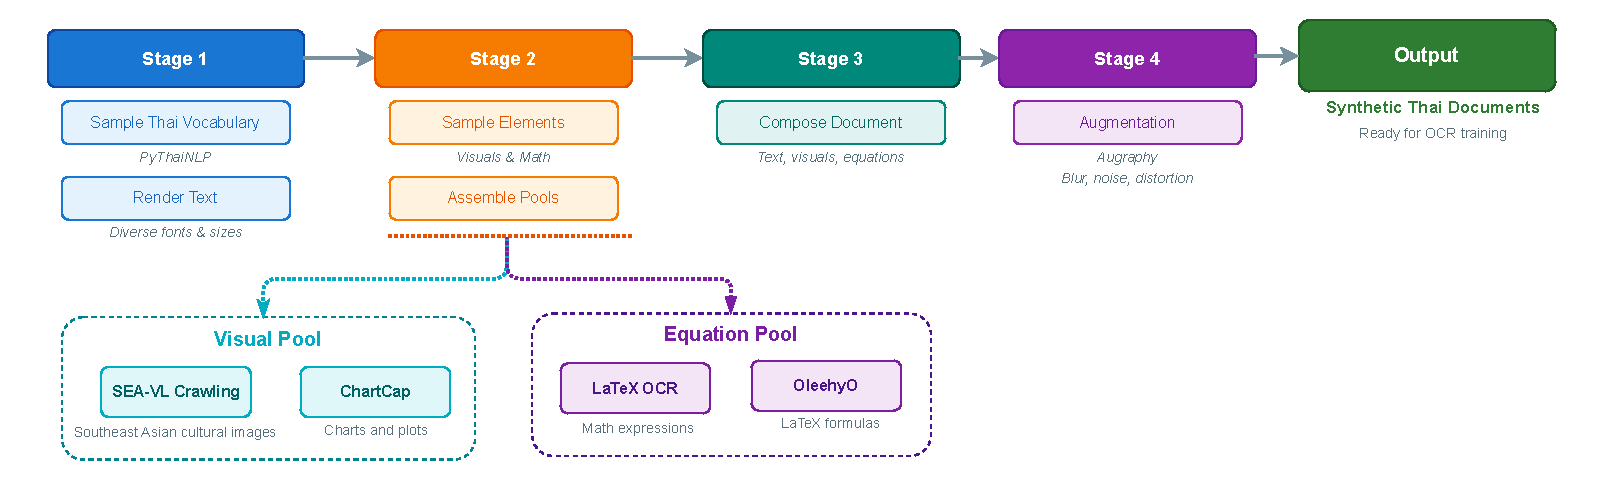
\includegraphics[width=\linewidth]{picture/synthetic_document_gen.pdf}
    \caption{Multi-stage pipeline for generating synthetic Thai document images for OCR training.}
    \label{fig:dataset_synth_ocr}
\end{figure}

\subparagraph{Stage 1} Thai vocabulary is randomly sampled from PyThaiNLP \citep{phatthiyaphaibun-etal-2023-pythainlp} and rendered using diverse font families and font sizes to increase robustness to typographic variation and low-frequency lexical forms

\subparagraph{Stage 2} Visual elements are sampled from SEA-VL Crawling\footnote{\url{https://huggingface.co/datasets/SEACrowd/sea-vl_crawling}} \citep{cahyawijaya2025crowdsourcecrawlgeneratecreating}, which contains culturally relevant images from Southeast Asia, and from ChartCap\footnote{\url{https://huggingface.co/datasets/junyoung-00/ChartCap}} \citep{lim2025chartcapmitigatinghallucinationdense} to provide real-world charts and plots for training layout and figure understanding.

\subparagraph{Stage 3} Mathematical expressions are sampled from LaTeX OCR\footnote{\url{https://huggingface.co/datasets/linxy/LaTeX_OCR}} and OleehyO LaTeX Formulas\footnote{\url{https://huggingface.co/datasets/lamm-mit/OleehyO-latex-formulas}} to improve recognition of equation structures and symbolic layouts.

\subparagraph{Stage 4} We apply document-level image augmentation using Augraphy\footnote{\url{https://github.com/sparkfish/augraphy}} \citep{augraphy_paper} to simulate real-world acquisition artifacts such as blur, noise, compression, illumination variation, and geometric distortion. This step increases visual diversity and improves robustness to degraded scanning and photographic conditions.

These components are combined to generate documents containing mixed textual, mathematical, and visual content with controlled layout variation and Thai-specific linguistic features.

% To support this unified formulation, all training annotations are normalized into a structured, multimodal representation that captures both textual content and document layout. Specifically, the training data employ the following representations:

% \begin{itemize}
%     \item \texttt{Markdown} for narrative content, paragraph text, and inline formatting.
    
%     \item \texttt{HTML} for complex tables and structured layouts requiring explicit row and column semantics.
    
%     \item \texttt{\textless figure\textgreater} tags for non-textual visual elements such as charts, diagrams, and illustrations, accompanied by descriptive captions when available.
    
%     \item \texttt{\textless page\_number\textgreater} tags to explicitly encode page numbers as they appear in the visual layout, preserving pagination information in multi-page documents.
    
%     \item \textbf{Checkbox and form control normalization}, in which checkboxes and radio buttons are mapped to standardized Unicode symbols (\ding{110}, \ding{51}, \ding{55}) to ensure consistent representation across heterogeneous form designs.
    
%     \item \textbf{Mathematical expression normalization}, where detected equations are converted into properly formatted \LaTeX{} syntax to preserve mathematical semantics and enable downstream reuse.
% \end{itemize}

% This unified data representation allows Typhoon OCR V1.5 to learn a consistent mapping from visual document input to structured, semantically rich output, regardless of document domain or layout complexity. By consolidating multiple output formats into a single prompt and representation scheme, the model achieves improved robustness, reduced inference overhead, and more predictable behavior in real-world document processing pipelines.


% \subsection{Dataset statistic}
% Figure~\ref{fig:dataset_dis2} shows the distribution of the training dataset in version 1.5. We followed same pipline in first version but improve more accuracy by labeling with Qwen3-VL ~\citep{bai2025qwen3vltechnicalreport} and dots.ocr ~\citep{li2025dotsocrmultilingualdocumentlayout} which are powerful model in multilingual support Thai language.


% \begin{figure}[htbp]
%     \centering
%     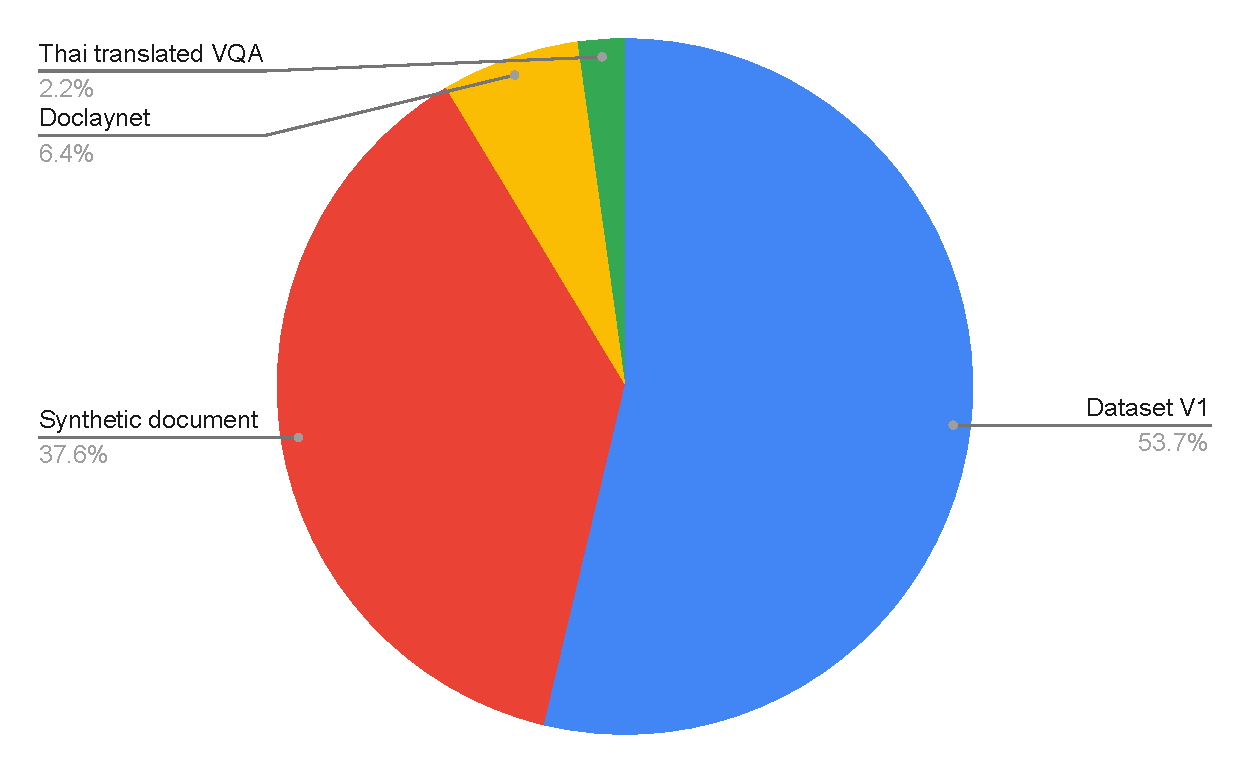
\includegraphics[width=0.7\textwidth]{picture/chartv3.pdf}
%     \caption{Training dataset distribution used for fine-tuning Typhoon OCR}
%     \label{fig:dataset_dis2}
% \end{figure}


% Figure~\ref{fig:dataset_dis2} illustrates the distribution of our training dataset by sources in version 1.5, which comprises diverse document types in both Thai and English. The dataset is composed of the following major categories:

% \begin{itemize}
%     \item \textbf{Dataset V1 (53.7\%):} 
%     \item \textbf{Thai translated VQA (2.2\%):} we utilize typhoon translated to translated English to Thai. sample random from The Cauldron\footnote{\url{https://huggingface.co/datasets/HuggingFaceM4/the_cauldron}}
%     \item \textbf{DocLayNet-v1.2 (6.4\%)} sample random from The Cauldron\footnote{\url{https://huggingface.co/datasets/docling-project/DocLayNet-v1.2}}

%     \item \textbf{Synthetic document (37.6\%):} we use multi datasets to combined into document such as LaTeX OCR \footnote{\url{https://huggingface.co/datasets/linxy/LaTeX_OCR }} , OleehyO-latex-formulas \footnote{\url{https://huggingface.co/datasets/lamm-mit/OleehyO-latex-formulas }}, ChartCap \footnote{\url{https://huggingface.co/datasets/junyoung-00/ChartCap }}, sea-vl crawling \footnote{\url{https://huggingface.co/datasets/SEACrowd/sea-vl_crawling}} and Thai vocab dictionary~\citep{phatthiyaphaibun-etal-2023-pythainlp}
% \end{itemize}

% \subsection{Dataset Statistics}

% Figure~\ref{fig:dataset_dis2} presents the distribution of the training dataset used for fine-tuning Typhoon OCR V1.5. We follow the same overall data construction pipeline as in version~1, while improving annotation quality through the use of more recent multilingual vision--language models. In particular, labeling is enhanced using Qwen3-VL~\citep{bai2025qwen3vltechnicalreport} and Dots.OCR~\citep{li2025dotsocrmultilingualdocumentlayout}, both of which demonstrate strong performance on multilingual document understanding and Thai language content.

% \begin{figure}[htbp]
%     \centering
%     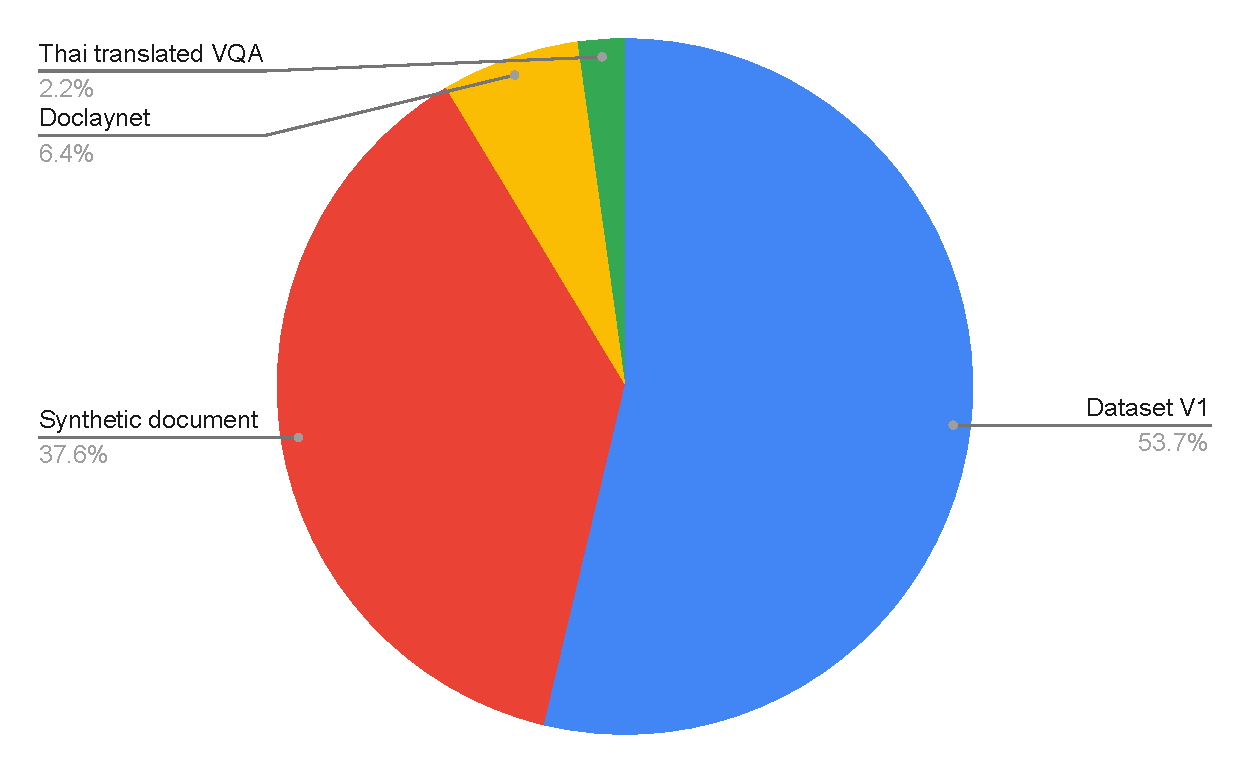
\includegraphics[width=0.7\textwidth]{picture/chartv3.pdf}
%     \caption{Training dataset distribution used for fine-tuning Typhoon OCR V1.5}
%     \label{fig:dataset_dis2}
% \end{figure}

% Figure~\ref{fig:dataset_dis2} further illustrates the distribution of the training data by source in version~1.5. The dataset consists of a diverse mixture of Thai and English document types and is composed of the following major categories:

% \begin{itemize}
%     \item \textbf{Typhoon OCR V1 Dataset (53.7\%):}  
%     The original training data used in version~1, retained to preserve continuity and stability across model iterations.

%     \item \textbf{Thai-Translated VQA Data (2.2\%):}  
%     Vision--question answering samples derived from The Cauldron dataset\footnote{\url{https://huggingface.co/datasets/HuggingFaceM4/the_cauldron}}, translated from English to Thai using the Typhoon translation system. Random subsampling is applied to maintain balance and diversity.

%     \item \textbf{DocLayNet-v1.2 (6.4\%):}  
%     A randomly sampled subset of DocLayNet-v1.2\footnote{\url{https://huggingface.co/datasets/docling-project/DocLayNet-v1.2}}, providing high-quality layout annotations for structured documents.

%     \item \textbf{Synthetic Document Data (37.6\%):}  
%     A collection of synthetically generated documents constructed by combining multiple public datasets, including LaTeX OCR\footnote{\url{https://huggingface.co/datasets/linxy/LaTeX_OCR}}, OleehyO LaTeX Formulas\footnote{\url{https://huggingface.co/datasets/lamm-mit/OleehyO-latex-formulas}}, ChartCap\footnote{\url{https://huggingface.co/datasets/junyoung-00/ChartCap}}, SEA-VL Crawling\footnote{\url{https://huggingface.co/datasets/SEACrowd/sea-vl_crawling}}, and Thai vocabulary resources from PyThaiNLP~\citep{phatthiyaphaibun-etal-2023-pythainlp}. These sources enable controlled generation of documents containing mathematical expressions, charts, structured layouts, and Thai-specific linguistic content.
% \end{itemize}

% Overall, the expanded and diversified dataset in version~1.5 strengthens the model's ability to generalize across document domains, layout complexities, and language conditions, while maintaining compatibility with the training distribution of the initial release.

% \subsection{Dataset Statistics}

% Figure~\ref{fig:dataset_dis2} summarizes the training corpus used to fine-tune Typhoon OCR V1.5. The overall data construction pipeline follows that of version~1, while annotation quality is improved through the use of more recent multilingual vision--language models. In particular, labeling is performed using Qwen3-VL~\citep{bai2025qwen3vltechnicalreport} and Dots.OCR~\citep{li2025dotsocrmultilingualdocumentlayout}, which provide stronger multilingual and Thai document understanding capabilities.


% \begin{figure}[htbp]
%     \centering
%     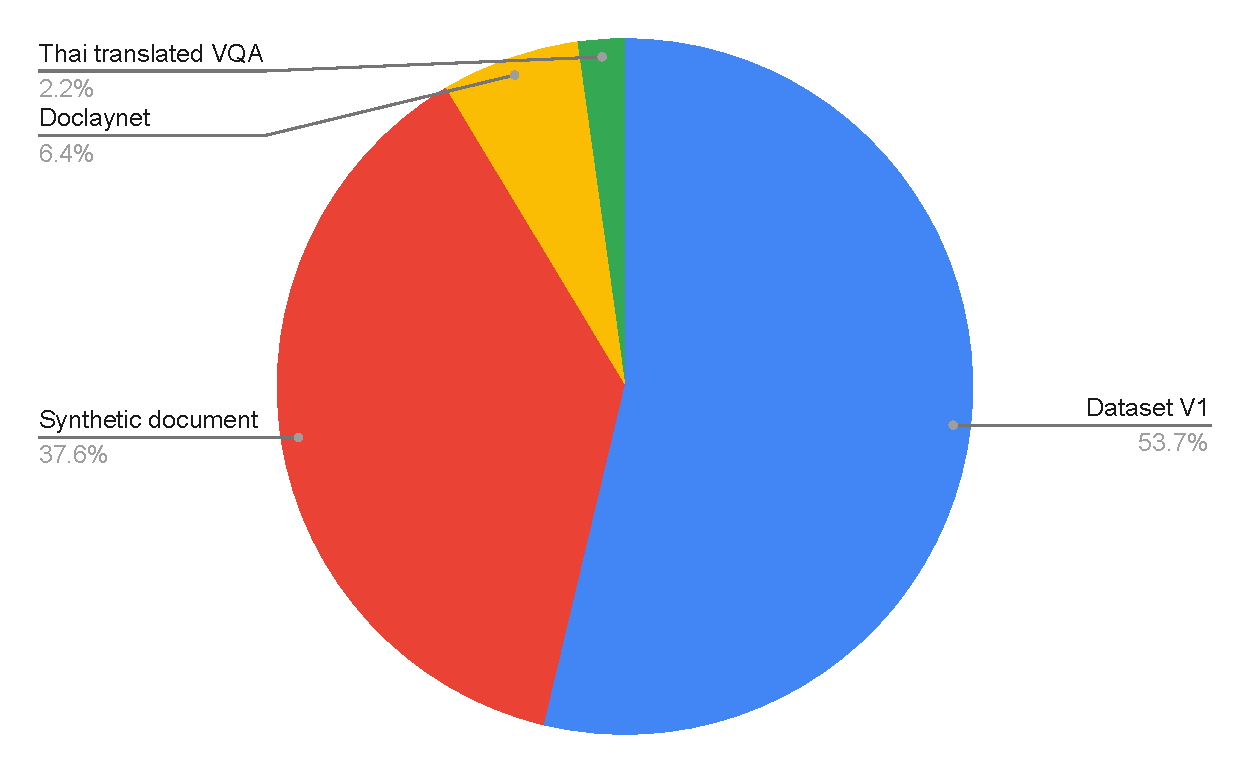
\includegraphics[width=0.7\textwidth]{picture/chartv3.pdf}
%     \caption{Training dataset distribution for Typhoon OCR V1.5}
%     \label{fig:dataset_dis2}
% \end{figure}


% As shown in Figure~\ref{fig:dataset_dis2}, the training corpus consists of a mixture of Thai and English document sources. More than half of the data (53.7\%) is retained from the Typhoon OCR V1 training set to ensure continuity across model versions. An additional 2.2\% comprises Thai-translated vision--question answering samples derived from The Cauldron dataset\footnote{\url{https://huggingface.co/datasets/HuggingFaceM4/the_cauldron}}. These samples are translated from English to Thai using the Typhoon translation model\footnote{\url{https://huggingface.co/scb10x/typhoon-translate-4b}}, with random subsampling applied to maintain dataset balance.


% Structured document supervision is supplemented using a subset of DocLayNet-v1.2\footnote{\url{https://huggingface.co/datasets/docling-project/DocLayNet-v1.2}}, contributing 6.4\% of the corpus. Synthetic data accounts for 37.6\% of the training set and is generated by combining multiple public sources, including LaTeX OCR\footnote{\url{https://huggingface.co/datasets/linxy/LaTeX_OCR}}, OleehyO LaTeX Formulas\footnote{\url{https://huggingface.co/datasets/lamm-mit/OleehyO-latex-formulas}}, ChartCap\footnote{\url{https://huggingface.co/datasets/junyoung-00/ChartCap}}, SEA-VL Crawling\footnote{\url{https://huggingface.co/datasets/SEACrowd/sea-vl_crawling}}, and Thai vocabulary resources from PyThaiNLP~\citep{phatthiyaphaibun-etal-2023-pythainlp}. These sources support controlled generation of documents containing mathematical expressions, charts, structured layouts, and Thai-specific linguistic content. The expanded and diversified dataset in version~1.5 improves coverage of document domains and layout complexity while maintaining compatibility with the training distribution of the initial release.

\subsubsection{Dataset Statistics}

\Cref{fig:dataset_dis2} summarizes the statistics of training corpus used to fine-tune Typhoon OCR V1.5. The training corpus consists of a mixture of Thai and English document sources.

\begin{figure}[htbp]
    \centering
    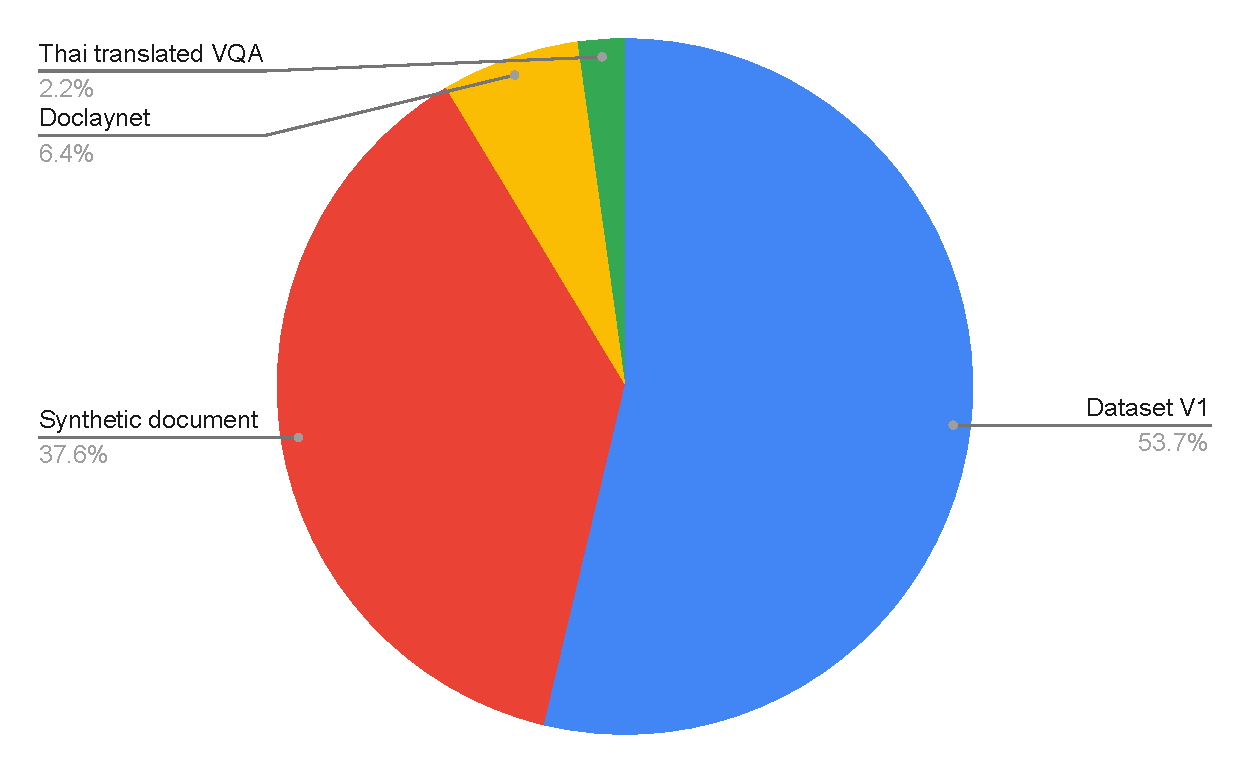
\includegraphics[width=0.6\textwidth]{picture/chartv3.pdf}
    \caption{Training dataset distribution for Typhoon OCR V1.5}
    \label{fig:dataset_dis2}
\end{figure}

The largest portion of the dataset (53.7\%) is retained from the \textbf{Typhoon OCR V1 training corpus} to ensure performance consistency across model versions and preserve coverage of previously observed document distributions. The dataset also include VQA samples from The Cauldron, constituting 2.2\% of the overall training corpus and is intentionally kept as a small fraction, as Typhoon OCR is primarily designed for document understanding rather than general-purpose VQA. The inclusion of this subset aims to preserve basic multimodal reasoning capabilities and mitigate catastrophic forgetting of generic vision-language knowledge during document-centric fine-tuning.

Structured document supervision is supplemented using a subset of DocLayNet-v1.2\footnote{\url{https://huggingface.co/datasets/docling-project/DocLayNet-v1.2}} \citep{doclaynet2022}, contributing 6.4\% of the corpus and providing high-quality annotations for layout segmentation and structural regions. The remaining 37.6\% consists of synthetic documents generated using the pipeline described in the previous section. We intentionally maintain a substantial synthetic portion to compensate for the limited availability of annotated Thai documents containing equations and charts. In total, the
training corpus contains 155,403 document samples.

% Overall, the expanded dataset in version~1.5 improves coverage of document domains, visual complexity, and language phenomena while maintaining compatibility with the training distribution of the initial release.



% \subsection{Training Settings}
% We conducted supervised fine-tuning (SFT) based on the Qwen3-VL models (2B) using full-parameter fine-tuning. The training code was adapted from the Axolotl GitHub repository\footnote{\url{https://github.com/axolotl-ai-cloud/axolotl}}. For data preprocessing, we categorize into 2 cases, in case of image small than 1,800 pixel we training with original resolution and bigger than that we then resize with same aspect ratio to 1,800. The models were trained with a total sequence length of 16,384 tokens on 4 GPUs with 80GB of memory each. Training was performed for 2 epochs, and we selected the best checkpoint based on performance on the evaluation set.
% \subsection{Training Settings}

% We perform supervised fine-tuning (SFT) on the Qwen3-VL 2B vision--language model using full-parameter optimization. The training pipeline is adapted from the open-source \texttt{Axolotl} repository\footnote{\url{https://github.com/axolotl-ai-cloud/axolotl}}, with modifications to support long-context multimodal inputs and document-centric training objectives.

% For data preprocessing, we adopt a resolution-aware strategy to balance visual fidelity and computational efficiency. Input images are processed under two cases: images with a maximum dimension smaller than 1{,}800 pixels are retained at their original resolution, while larger images are resized to a maximum width of 1{,}800 pixels while preserving the original aspect ratio.

% The model is trained with a total sequence length of 16{,}384 tokens to accommodate long-form documents and complex layouts. Training is conducted on four GPUs, each equipped with 80\,GB of memory. Fine-tuning is performed for two epochs, and the final checkpoint is selected based on performance on a held-out evaluation set. This configuration enables stable optimization while maintaining efficient training and inference characteristics.

% \subsection{Training Settings}

% Typhoon OCR V1.5 is trained via supervised fine-tuning on the Qwen3-VL 2B vision--language model using full-parameter optimization. The training pipeline is based on the open-source \texttt{Axolotl} framework\footnote{\url{https://github.com/axolotl-ai-cloud/axolotl}}, with extensions to support long-context multimodal inputs and document-centric training objectives.

% During preprocessing, a resolution-aware strategy is applied to balance visual fidelity and computational efficiency. Images with a maximum dimension below 1{,}800 pixels are retained at their original resolution, while larger images are resized to a maximum width of 1{,}800 pixels with aspect ratio preserved.

% The maximum sequence length is set to 16{,}384 tokens to accommodate long documents and complex layouts. Training is performed on four GPUs with 80\,GB of memory each for two epochs. The final checkpoint is selected based on validation performance, providing a balance between optimization stability and efficient training and inference.

\subsection{Experimental Setup}
\subsubsection{Training}

Typhoon OCR V1.5 is trained using full-parameter SFT on the Qwen3-VL 2B VLM. The training framework is based on the open-source \texttt{Axolotl} framework\footnote{\url{https://github.com/axolotl-ai-cloud/axolotl}} \citep{axolotl}, with extensions to support long-context multimodal inputs and document-centric training objectives.

During preprocessing, a resolution-aware strategy is applied to balance visual fidelity and computational efficiency. Images with a maximum dimension below 1,800 pixels are \emph{retained} at their original resolution, while larger images are resized to a maximum width of 1,800 pixels with aspect ratio preserved. The maximum sequence length is set to 16,384 tokens to accommodate long documents and complex layouts.

Training is performed on 4$\times$H100 GPUs for two epochs, and the final checkpoint is selected based on validation performance. Quantization-aware training \citep{Jacob_2018_CVPR} is applied during fine-tuning to expose the model to quantization effects, enabling efficient low-precision inference with only limited impact on accuracy.


% \subsection{Evaluation and Results}

% \subsubsection{Evaluation Setup}
% To assess the performance of Typhoon OCR, we use same matric with typhoon v1.

% We evaluate Typhoon OCR in one prompt settings. We compare Typhoon OCR against two state-of-the-art vision-language baselines:

% \begin{itemize}
%     \item \textbf{Typhoon 7B V1} (released )
%     \item \textbf{GPT-5} (released )
%     \item \textbf{Gemini 2.5 Pro} (released )
% \end{itemize}

% \subsection{Evaluation and Results}
% \subsubsection{Evaluation Setup}
% To evaluate the performance of Typhoon OCR V1.5, we adopt the same evaluation metrics and protocols used for Typhoon OCR V1, ensuring comparability across model versions. Specifically, we report BLEU, ROUGE-L, and Levenshtein Distance to assess lexical accuracy, structural similarity, and character-level fidelity, respectively.

% \subsubsection{Evaluation Datasets}
% For evaluation, we reuse the held-out test sets from Typhoon OCR V1 to ensure direct comparability between model versions. These datasets are further refined through additional human annotation and quality control to reduce noise and improve annotation consistency. In addition, we introduce two newly curated evaluation datasets focusing on infographic-style documents and handwritten forms, both created and validated by human annotators.

% The evaluation datasets include the following categories:

% \begin{itemize}
%     \item \textbf{Thai Financial Reports:}  
%     Structured financial documents originally used in version~1 and subsequently refined through human review. These documents contain tables, charts, and mixed Thai--English content.

%     \item \textbf{Thai Government Forms:}  
%     Administrative forms reused from version~1 with enhanced human quality control. The dataset includes dense layouts, handwritten annotations, and domain-specific terminology.

%     \item \textbf{Thai Books:}  
%     Long-form documents retained from version~1 and further cleaned through human verification. These documents contain extended textual passages interleaved with diagrams, illustrations, and embedded figures.

%     \item \textbf{Infographics:}  
%     A newly introduced evaluation set consisting of unstructured or loosely structured infographic-style documents with heterogeneous layouts and prominent visual elements.

%     \item \textbf{Handwritten Forms:}  
%     A newly curated dataset of forms containing a mixture of handwritten and printed text, such as banking and administrative forms, designed to evaluate robustness under realistic handwriting conditions.
% \end{itemize}

% \begin{table}[htbp]
% \centering
% \small
% \begin{tabular}{lccccc}
% \toprule
% \textbf{Task} & \textbf{Metric} & \textbf{Typhoon7B v1} & \textbf{Typhoon2B v1.5} & \textbf{Gemini2.5-pro} & \textbf{GPT-5} \\
% \midrule
% Thai Books             & BLEU & 0.708 & \textbf{0.746} & 0.512 & 0.710 \\
% Thai Government Forms  & BLEU & 0.849 & \textbf{0.870} & 0.797 & 0.569 \\
% Thai Financial Reports & BLEU & \textbf{0.849} & 0.819 & 0.657 & 0.457 \\
% Infographics           & BLEU & 0.246 & 0.408 & \textbf{0.465} & 0.297 \\
% Handwriting Forms      & BLEU & 0.321 & 0.522 & \textbf{0.594} & 0.368 \\
% Others                 & BLEU & 0.376 & 0.499 & \textbf{0.603} & 0.352 \\
% \midrule
% Average                & BLEU & 0.558 & \textbf{0.644} & 0.605 & 0.459 \\
% \bottomrule
% \end{tabular}
% \caption{BLEU scores by document category (higher is better).}
% \label{tab:bleu_by_task}
% \end{table}

% \begin{table}[htbp]
% \centering
% \small
% \begin{tabular}{lccccc}
% \toprule
% \textbf{Task} & \textbf{Metric} & \textbf{Typhoon7B v1} & \textbf{Typhoon2B v1.5} & \textbf{Gemini2.5-pro} & \textbf{GPT-5} \\
% \midrule
% Thai Books             & ROUGE\_L & 0.871 & \textbf{0.949} & 0.676 & 0.922 \\
% Thai Government Forms  & ROUGE\_L & 0.942 & \textbf{0.967} & 0.894 & 0.706 \\
% Thai Financial Reports & ROUGE\_L & \textbf{0.933} & 0.910 & 0.757 & 0.603 \\
% Infographics           & ROUGE\_L & 0.373 & 0.527 & \textbf{0.677} & 0.481 \\
% Handwriting Forms      & ROUGE\_L & 0.454 & 0.645 & \textbf{0.739} & 0.514 \\
% Others                 & ROUGE\_L & 0.541 & 0.645 & \textbf{0.716} & 0.482 \\
% \midrule
% Average                & ROUGE\_L & 0.686 & \textbf{0.774} & 0.743 & 0.618 \\
% \bottomrule
% \end{tabular}
% \caption{ROUGE-L scores by document category (higher is better).}
% \label{tab:rouge_by_task}
% \end{table}

% \begin{table}[htbp]
% \centering
% \small
% \begin{tabular}{lccccc}
% \toprule
% \textbf{Task} & \textbf{Metric} & \textbf{Typhoon7B v1} & \textbf{Typhoon2B v1.5} & \textbf{Gemini2.5-pro} & \textbf{GPT-5} \\
% \midrule
% Thai Books             & LEVENSHTEIN & 0.136 & \textbf{0.053} & 0.334 & 0.084 \\
% Thai Government Forms  & LEVENSHTEIN & 0.065 & \textbf{0.035} & 0.096 & 0.267 \\
% Thai Financial Reports & LEVENSHTEIN & 0.082 & \textbf{0.079} & 0.256 & 0.356 \\
% Infographics           & LEVENSHTEIN & 0.671 & 0.544 & \textbf{0.380} & 0.561 \\
% Handwriting Forms      & LEVENSHTEIN & 0.556 & 0.416 & \textbf{0.327} & 0.533 \\
% Others                 & LEVENSHTEIN & 0.480 & 0.377 & \textbf{0.342} & 0.540 \\
% \midrule
% Average                & LEVENSHTEIN & 0.332 & \textbf{0.251} & 0.289 & 0.390 \\
% \bottomrule
% \end{tabular}
% \caption{Levenshtein distance by document category (lower is better).}
% \label{tab:lev_by_task}
% \end{table}

\subsubsection{Evaluation}

\paragraph{Protocol and Metrics} We evaluate Typhoon OCR V1.5 using the same metrics and protocols as V1 (\Cref{sec:v1_eval}) to ensure comparability across model iterations. Namely, we report \textbf{BLEU}, \textbf{ROUGE-L}, and \textbf{Levenshtein distance} to measure lexical accuracy, sequence-level structural similarity, and character-level transcription fidelity, respectively.

\paragraph{Benchmark}

Evaluation is conducted on held-out test sets from Typhoon OCR V1, which are further refined through additional human annotation and quality control to reduce noise and improve consistency. In addition, two new evaluation sets are introduced to assess performance on document types that were underrepresented in V1.

The evaluation corpus comprises six categories:
\begin{enumerate}
    \item \textbf{Thai Books:} Consist of long-form documents with extended text interleaved with figures and illustrations.
    \item \textbf{Thai Government Forms:} Reused from V1 with enhanced human verification. This benchmark includes dense layouts, tables, charts, and handwritten annotations.
    \item \textbf{Thai Financial Reports:} Also reused from V1 with enhanced human verification.
    \item \textbf{Infographics:} Contain loosely structured documents with prominent visual elements.
    \item \textbf{Handwritten Forms:} Consist of administrative and financial forms that combine handwritten and printed text.
    \item \textbf{Others:} A diverse collection of semi-structured and unstructured documents, including receipts, bills, tickets, and miscellaneous transactional records.
\end{enumerate}
% \begin{table}[htbp]
% \centering
% \renewcommand*{\arraystretch}{1.2}
% \resizebox{\linewidth}{!}{
% \begin{tabular}{lcccc}
% \toprule
% \textbf{Task} & \textbf{Typhoon OCR V1 7B} & \textbf{Typhoon OCR V1.5 2B} & \textbf{Gemini 2.5 Pro} & \textbf{GPT-5} \\
% \midrule
% Thai Books             & 0.708 & \textbf{0.746} & 0.512 & 0.710 \\
% Thai Government Forms  & 0.849 & \textbf{0.870} & 0.797 & 0.569 \\
% Thai Financial Reports & \textbf{0.849} & 0.819 & 0.657 & 0.457 \\
% Infographics           & 0.246 & 0.408 & \textbf{0.465} & 0.297 \\
% Handwriting Forms      & 0.321 & 0.522 & \textbf{0.594} & 0.368 \\
% Others                 & 0.376 & 0.499 & \textbf{0.603} & 0.352 \\
% \midrule
% \textbf{Average}                & 0.558 & \textbf{0.644} & 0.605 & 0.459 \\
% \bottomrule
% \end{tabular}
% }
% \caption{BLEU scores by document category (higher is better).}
% \label{tab:bleu_by_task}
% \end{table}
\begin{table}[htbp]
\centering
\renewcommand*{\arraystretch}{1.2}
\resizebox{\linewidth}{!}{
\begin{tabular}{lcccc}
\toprule
\textbf{Task} & \textbf{Gemini 2.5 Pro} & \textbf{GPT-5} & \textbf{Typhoon OCR V1 7B} & \textbf{Typhoon OCR V1.5 2B} \\
\midrule
Thai Books             & 0.512 & 0.710 & 0.708 & \textbf{0.746} \\
Thai Government Forms  & 0.797 & 0.569 & 0.849 & \textbf{0.870} \\
Thai Financial Reports & 0.657 & 0.457 & \textbf{0.849} & 0.819 \\
Infographics           & \textbf{0.465} & 0.297 & 0.246 & 0.408 \\
Handwriting Forms      & \textbf{0.594} & 0.368 & 0.321 & 0.522 \\
Others                 & \textbf{0.603} & 0.352 & 0.376 & 0.499 \\
\midrule
\textbf{Average}       & 0.605 & 0.459 & 0.558 & \textbf{0.644} \\
\bottomrule
\end{tabular}
}
\caption{BLEU scores by document category (higher is better).}
\label{tab:bleu_by_task}
\end{table}
% \begin{table}[htbp]
% \centering
% \renewcommand*{\arraystretch}{1.2}
% \resizebox{\linewidth}{!}{
% \begin{tabular}{lcccc}
% \toprule
% \textbf{Task} & \textbf{Typhoon OCR V1 7B} & \textbf{Typhoon OCR V1.5 2B} & \textbf{Gemini 2.5 Pro} & \textbf{GPT-5} \\
% \midrule
% Thai Books             & 0.871 & \textbf{0.949} & 0.676 & 0.922 \\
% Thai Government Forms  & 0.942 & \textbf{0.967} & 0.894 & 0.706 \\
% Thai Financial Reports & \textbf{0.933} & 0.910 & 0.757 & 0.603 \\
% Infographics           & 0.373 & 0.527 & \textbf{0.677} & 0.481 \\
% Handwriting Forms      & 0.454 & 0.645 & \textbf{0.739} & 0.514 \\
% Others                 & 0.541 & 0.645 & \textbf{0.716} & 0.482 \\
% \midrule
% \textbf{Average}                & 0.686 & \textbf{0.774} & 0.743 & 0.618 \\
% \bottomrule
% \end{tabular}
% }
% \caption{ROUGE-L scores by document category (higher is better).}
% \label{tab:rouge_by_task}
% \end{table}
\begin{table}[htbp]
\centering
\renewcommand*{\arraystretch}{1.2}
\resizebox{\linewidth}{!}{
\begin{tabular}{lcccc}
\toprule
\textbf{Task} & \textbf{Gemini 2.5 Pro} & \textbf{GPT-5} & \textbf{Typhoon OCR V1 7B} & \textbf{Typhoon OCR V1.5 2B} \\
\midrule
Thai Books             & 0.676 & 0.922 & 0.871 & \textbf{0.949} \\
Thai Government Forms  & 0.894 & 0.706 & 0.942 & \textbf{0.967} \\
Thai Financial Reports & 0.757 & 0.603 & \textbf{0.933} & 0.910 \\
Infographics           & \textbf{0.677} & 0.481 & 0.373 & 0.527 \\
Handwriting Forms      & \textbf{0.739} & 0.514 & 0.454 & 0.645 \\
Others                 & \textbf{0.716} & 0.482 & 0.541 & 0.645 \\
\midrule
\textbf{Average}       & 0.743 & 0.618 & 0.686 & \textbf{0.774} \\
\bottomrule
\end{tabular}
}
\caption{ROUGE-L scores by document category (higher is better).}
\label{tab:rouge_by_task}
\end{table}


% \begin{table}[htbp]
% \centering
% \renewcommand*{\arraystretch}{1.2}
% \resizebox{\linewidth}{!}{
% \begin{tabular}{lcccc}
% \toprule
% \textbf{Task} & \textbf{Typhoon OCR V1 7B} & \textbf{Typhoon OCR V1.5 2B} & \textbf{Gemini 2.5 Pro} & \textbf{GPT-5} \\
% \midrule
% Thai Books             & 0.136 & \textbf{0.053} & 0.334 & 0.084 \\
% Thai Government Forms  & 0.065 & \textbf{0.035} & 0.096 & 0.267 \\
% Thai Financial Reports & 0.082 & \textbf{0.079} & 0.256 & 0.356 \\
% Infographics           & 0.671 & 0.544 & \textbf{0.380} & 0.561 \\
% Handwriting Forms      & 0.556 & 0.416 & \textbf{0.327} & 0.533 \\
% Others                 & 0.480 & 0.377 & \textbf{0.342} & 0.540 \\
% \midrule
% \textbf{Average}                & 0.332 & \textbf{0.251} & 0.289 & 0.390 \\
% \bottomrule
% \end{tabular}
% }
% \caption{Levenshtein distance by document category (lower is better).}
% \label{tab:lev_by_task}
% \end{table}
\begin{table}[htbp]
\centering
\renewcommand*{\arraystretch}{1.2}
\resizebox{\linewidth}{!}{
\begin{tabular}{lcccc}
\toprule
\textbf{Task} & \textbf{Gemini 2.5 Pro} & \textbf{GPT-5} & \textbf{Typhoon OCR V1 7B} & \textbf{Typhoon OCR V1.5 2B} \\
\midrule
Thai Books             & 0.334 & 0.084 & 0.136 & \textbf{0.053} \\
Thai Government Forms  & 0.096 & 0.267 & 0.065 & \textbf{0.035} \\
Thai Financial Reports & 0.256 & 0.356 & 0.082 & \textbf{0.079} \\
Infographics           & \textbf{0.380} & 0.561 & 0.671 & 0.544 \\
Handwriting Forms      & \textbf{0.327} & 0.533 & 0.556 & 0.416 \\
Others                 & \textbf{0.342} & 0.540 & 0.480 & 0.377 \\
\midrule
\textbf{Average}       & 0.289 & 0.390 & 0.332 & \textbf{0.251} \\
\bottomrule
\end{tabular}
}
\caption{Levenshtein distance by document category (lower is better).}
\label{tab:lev_by_task}
\end{table}



% \subsection{Results and Discussion}

% Tables~\ref{tab:bleu_by_task}--\ref{tab:rouge_by_task} report the performance of Typhoon OCR v1.5 compared with Typhoon OCR v1 and two state-of-the-art vision--language models across multiple Thai document categories.

% Despite having substantially fewer parameters (2B vs.\ 7B), Typhoon OCR v1.5 consistently improves upon the first-generation model across all evaluation metrics. In terms of BLEU, the average score increases from 0.558 to 0.644, indicating improved word- and phrase-level accuracy. Similarly, ROUGE-L improves from 0.686 to 0.774, reflecting better preservation of sequence structure and contextual alignment in the generated outputs. At the character level, the average Levenshtein distance decreases from 0.332 to 0.251 (lower is better), demonstrating a reduction in fine-grained transcription errors.

% Performance gains are particularly pronounced on structured and visually complex documents. For Thai government forms, Typhoon OCR v1.5 achieves the best results across all three metrics (BLEU 0.870, ROUGE-L 0.967, and Levenshtein 0.035), outperforming both proprietary baselines. On Thai books, the model shows clear improvements in BLEU (0.746) and ROUGE-L (0.949), along with a substantial reduction in character-level errors, suggesting stronger handling of long and hierarchically structured text.

% The largest relative gains are observed on handwritten and mixed-media documents. For handwritten forms, BLEU improves from 0.321 to 0.522 and ROUGE-L from 0.454 to 0.645, highlighting the effectiveness of the updated handwriting recognition and form-field modeling. Infographics and other visually rich documents also benefit from the architectural and data improvements, with BLEU increasing from 0.246 to 0.408 and ROUGE-L from 0.373 to 0.527, indicating better figure recognition and layout understanding.

% Overall, these results demonstrate that Typhoon OCR v1.5 achieves stronger accuracy and robustness across diverse Thai document types, while remaining parameter-efficient relative to both its predecessor and larger proprietary models.

% \subsection{Results and Discussion}

% \textbf{Results.}  
% Tables~\ref{tab:bleu_by_task}--\ref{tab:rouge_by_task} report the performance of Typhoon OCR V1.5 in comparison with Typhoon OCR V1 and two vision--language baselines across multiple Thai document categories.

% Although Typhoon OCR V1.5 uses substantially fewer parameters (2B versus 7B), it shows consistent improvements over the first-generation model across all evaluation metrics. The average BLEU score increases from 0.558 to 0.644, indicating improved word- and phrase-level accuracy. ROUGE-L improves from 0.686 to 0.774, reflecting better preservation of sequential structure, while the average Levenshtein distance decreases from 0.332 to 0.251, indicating fewer character-level errors.

% Improvements are most pronounced on structured documents. On Thai government forms, Typhoon OCR V1.5 achieves the highest scores across all metrics (BLEU 0.870, ROUGE-L 0.967, and Levenshtein 0.035). On Thai books, performance increases in both BLEU (0.746) and ROUGE-L (0.949), accompanied by a reduction in character-level errors, suggesting improved handling of long-form and hierarchically structured content.

% Substantial gains are also observed on handwritten and visually complex documents. For handwritten forms, BLEU increases from 0.321 to 0.522 and ROUGE-L from 0.454 to 0.645. Infographic-style documents show similar trends, with BLEU improving from 0.246 to 0.408 and ROUGE-L from 0.373 to 0.527, indicating better handling of mixed visual and textual elements.

% Overall, these results indicate that Typhoon OCR V1.5 improves accuracy and robustness across diverse Thai document types while maintaining a significantly smaller model size than both its predecessor and larger vision--language baselines.

% \subsection{Results and Discussion}

% Tables~\ref{tab:bleu_by_task}--\ref{tab:lev_by_task} present a comparative evaluation of Typhoon OCR V1.5 against Typhoon OCR V1 and two large vision--language baselines across multiple Thai document categories. Rather than focusing solely on absolute metric values, we analyze how different model design choices affect performance across document types and deployment scenarios.

% A consistent trend across all metrics is that Typhoon OCR V1.5, despite its smaller parameter count (2B versus 7B), achieves higher average performance than Typhoon OCR V1. This result suggests that architectural simplification, unified prompting, and improved dataset construction contribute more to document understanding quality than model scale alone. For practitioners, this indicates that smaller, well-adapted models can be sufficient for Thai document processing tasks without incurring the latency and resource costs of larger systems.

% Performance improvements are most evident on structured documents such as Thai government forms and financial reports. In these domains, Typhoon OCR models outperform proprietary baselines on BLEU and ROUGE-L, while achieving lower Levenshtein distances. These results highlight the importance of explicit layout modeling and domain-aligned training data for documents with predictable structural patterns. For users working with administrative or financial documents, these findings suggest that Typhoon OCR is particularly well suited for high-precision extraction and downstream automation.

% In contrast, for visually complex categories such as infographics and handwritten forms, proprietary models achieve stronger character-level accuracy, as reflected by lower Levenshtein distances. However, Typhoon OCR V1.5 narrows this gap substantially relative to V1, indicating that dataset diversification and improved handwriting coverage are effective but not yet sufficient to fully address highly heterogeneous visual content. This observation underscores a practical trade-off: tasks emphasizing semantic structure and layout fidelity may favor Typhoon OCR, while tasks requiring fine-grained visual interpretation may benefit from further task-specific adaptation.

\subsection{Results and Discussion}

\Cref{tab:bleu_by_task,tab:rouge_by_task,tab:lev_by_task} report a comparative evaluation of Typhoon OCR V1.5 against Typhoon OCR V1 and two frontier VLM baselines across multiple Thai document categories. We analyze performance trends in relation to model design and document characteristics. Across all metrics, Typhoon OCR V1.5 achieves higher average performance than Typhoon OCR V1, despite having fewer parameters (2B versus 7B). This result indicates that improved data and training recipe have a greater impact on document extraction quality than model size alone. From a deployment perspective, the results suggest that compact, task-adapted models can provide strong performance while reducing computational overhead compared to \textit{one-size-fits-all} proprietary models.

Performance gains are most pronounced for structured document types, including Thai government forms and financial reports. In these categories, Typhoon OCR V1.5 consistently outperforms proprietary baselines on BLEU and ROUGE-L and achieves lower Levenshtein distances. This behavior reflects the benefit of explicit layout modeling and domain-aligned supervision for documents with regular structural patterns, which are common in administrative and financial workflows.

For visually heterogeneous categories such as infographics and handwritten forms, proprietary models achieve lower character-level error rates. Nevertheless, Typhoon OCR V1.5 substantially improves over V1, narrowing the gap in both lexical and structural metrics. This is an area for improvement that we aim to improve in future iterations.



% \subsection{Model Description}
% Typhoon OCR v1 is a bilingual, open-source Vision–Language Model (VLM) designed to address the limitations of conventional OCR systems for Thai and English documents. Traditional OCR pipelines are tightly coupled to character-level recognition and depend on heuristic post-processing, making them brittle in the presence of noise, layout irregularities, or complex document structures. In contrast, VLM-based OCR systems integrate visual perception with semantic understanding, enabling models to recognize text, infer structure, and interpret document content holistically. Typhoon OCR adopts this paradigm to deliver a unified, layout- and semantics-aware solution optimized for real-world document intelligence.

% Drawing inspiration from recent VLM-based OCR frameworks such as olmOCR, Typhoon OCR introduces a redesigned architecture that enhances robustness, broadens multilingual support, and improves structural fidelity. The model is engineered not only to transcribe text but also to generate richly structured outputs suitable for downstream applications that require document-level reasoning.

% \subsubsection{Design Principles}
% Typhoon OCR v1 is guided by three foundational design principles:

% \begin{itemize}
% \item \textbf{Robustness to Real-World Noise.}
% Documents encountered in practical settings--such as scanned forms, financial statements, receipts, and informal materials--often exhibit varying resolutions, compression artifacts, handwriting, or occlusions. Typhoon OCR incorporates visual encoders and fine-tuning strategies that improve resilience to such noise, ensuring consistent performance across heterogeneous input conditions.

% \item \textbf{Multilingual Capability.}
% The model provides dedicated, high-quality support for both Thai and English. Thai-specific visual and linguistic adaptations target issues such as stacked diacritics, variable orthographic composition, and the absence of explicit word boundaries, while English support ensures practicality for bilingual documents commonly used in administrative, academic, and commercial contexts.

% \item \textbf{Layout-Aware Understanding.}
% Rather than producing linear text, Typhoon OCR preserves document structure by explicitly modeling spatial relationships, hierarchical layout, and formatting cues. This enables faithful reconstruction of tables, lists, section hierarchies, figures, and other structural elements essential for downstream document analysis.
% \end{itemize}

% \subsubsection{Beyond Text Recognition: Structured and Semantic Outputs}

% Unlike traditional OCR systems that produce flat textual sequences, Typhoon~OCR~v1 generates structured representations that explicitly encode semantic units and document layout. This capability enables seamless integration with downstream applications such as retrieval-augmented generation (RAG), end-to-end document parsing, and content-based document retrieval.

% The model supports multiple output formats suited to different document components:

% \begin{itemize}
%     \item \textbf{Markdown} for general narrative text, preserving paragraph segmentation, headings, and inline annotations.
    
%     \item \textbf{HTML} for tables, capturing merged cells, nested structures, and complex grid configurations.
    
%     \item \textbf{Figure descriptors} represented using \texttt{<figure>} tags, combining visual and textual information for charts, diagrams, and embedded graphics.
% \end{itemize}

% Figure extraction follows a multi-stage interpretation process:

% \begin{itemize}
%     \item \textbf{Visual Observation}: Identification of salient visual elements such as objects, scenes, logos, and iconic symbols.
%     \item \textbf{Contextual Inference}: Determination of the figure's role or relevance within the surrounding document context.
%     \item \textbf{Embedded Text Recognition}: Extraction and transcription of Thai or English text appearing within the figure.
%     \item \textbf{Structural and Stylistic Parsing}: Characterization of chart types, diagrammatic structures, and stylistic conventions.
%     \item \textbf{Summary Generation}: Production of a concise, semantically coherent description suitable for document understanding and retrieval tasks.
% \end{itemize}

% This structured, multi-layered decoding framework enables Typhoon~OCR to move beyond conventional text extraction and to generate semantically rich, layout-aware document representations essential for advanced document-intelligence workflows.



% \subsubsection{Support for Diverse Document Modalities}

% Typhoon OCR v1 is optimized for both PDF and raster image inputs, enabling versatile deployment across diverse document ecosystems.

% PDF Parsing.
% For PDF files, the model leverages embedded metadata--such as reading order, bounding boxes, and vector-level annotations--to enhance recognition accuracy and maintain structural consistency. The integration of native PDF cues reduces ambiguities in layout interpretation and improves fidelity in table and figure reconstruction.

% Image Parsing.
% For image inputs lacking metadata, Typhoon OCR reconstructs layout using visual features and spatial relationships inferred from the document image. This capability ensures reliable parsing of photographs, scans, and camera-captured materials despite variable lighting or perspective distortions.

% \subsubsection{Support for Structured and Semi-Structured Documents}
% Typhoon OCR v1 is specifically optimized to handle structured documents such as financial reports, academic papers, books, technical manuals, and government forms. The model accurately processes hierarchical headings, multi-column layouts, footnotes, captioned figures, and complex tables. Its structured outputs are formatted for immediate use in downstream analytics, summarization, and automated knowledge extraction pipelines.

% In addition, the model provides strong performance on semi-structured and informal documents, including infographics, receipts, menus, tickets, and handwritten notes. Layout-aware decoding ensures that even irregular formats retain their essential relationships and semantics in the final output.
% \subsection{Data collection Pipeline and Training}
% \subsubsection{Dataset Preparation}
% We categorize the training dataset into two modes based on document structure and output requirements as shown in Table ~\ref{tab:modes-comparison}:
% \begin{table}[h]
% \centering
% \begin{tabular}{@{}p{4cm}p{5.5cm}p{5.5cm}@{}}
% \toprule
% \textbf{Feature} & \textbf{Default Mode} & \textbf{Structure Mode} \\
% \midrule
% \textbf{Intended Use} &
% Designed for unstructured or loosely structured documents such as infographics, receipts, menus, tickets, and handwritten notes. &
% Optimized for well-structured documents with complex layouts, including financial reports, academic papers, government forms, and books. \\
% \addlinespace

% \textbf{Layout Processing} &
% Focuses on content understanding and lightweight layout preservation suitable for flexible, informal documents. &
% Performs deep structural parsing with high-fidelity layout reconstruction, capturing complex hierarchies and semantic zones. \\
% \addlinespace

% \textbf{Output Format} &
% \texttt{Markdown} with inline layout and content preservation. &
% \begin{itemize}
%     \item \texttt{Markdown} for narrative and inline text.
%     \item \texttt{HTML} for complex tables and structured layout.
%     \item \texttt{<figure>} tags for visual elements like charts and diagrams.
% \end{itemize} \\
% \bottomrule
% \end{tabular}
% \caption{Comparison of Default Mode and Structure Mode in Typhoon OCR.}
% \label{tab:modes-comparison}
% \end{table}

% \subsubsection{Dataset statistic}
% test
% \subsubsection{Data collection Pipeline}
% test

% \subsection{Evaluation Setup}

% \section{Conclusion}

% This work addresses the problem of robust document understanding for Thai, a low-resource language with complex script properties and a wide variety of real-world document layouts. Existing OCR and vision--language systems either lack sufficient accuracy on Thai documents or remain inaccessible due to proprietary constraints, limiting both research progress and practical deployment.

% We introduced Typhoon OCR, an open-source vision--language document understanding system tailored for Thai and English documents. Through extensive experiments, we demonstrated that Typhoon OCR significantly improves text transcription accuracy, layout reconstruction, and semantic consistency compared to prior open-source approaches. Moreover, Typhoon OCR V1.5 achieves these improvements while substantially reducing model size and inference cost, outperforming both its predecessor and larger proprietary vision--language models across diverse document categories, including structured forms, handwritten documents, and visually complex layouts.

% The findings of this study have important implications for document intelligence in low-resource languages. They show that high-fidelity document understanding does not require training models from scratch or relying on closed systems; instead, it can be achieved through targeted adaptation of pretrained vision--language models combined with carefully designed data pipelines. This approach lowers the barrier to deploying reliable document understanding systems in resource-constrained and privacy-sensitive environments.

% Despite these advances, several limitations remain. Performance degrades on severely degraded inputs, such as low-resolution or heavily distorted images, and evaluation is currently limited to Thai and English. In addition, while transcription and layout fidelity are thoroughly evaluated, downstream document intelligence tasks are not yet comprehensively assessed.

% Building on this work, future research will explore extending Typhoon OCR to additional low-resource languages, improving robustness under adverse visual conditions, and integrating task-specific objectives for information extraction, question answering, and summarization. Further investigation into adaptive and hybrid inference strategies may also help balance efficiency and reasoning capacity across document types.

% In conclusion, Typhoon OCR demonstrates that open-source vision--language models can deliver accurate, efficient, and deployable document understanding for low-resource languages. We hope this work serves as a foundation for future research and accelerates the development of equitable document intelligence technologies worldwide.

\section{Conclusion}

This report introduces \textbf{Typhoon OCR}, a family of VLMs designed to address limitations in document understanding for Thai. The models consistently show improvements over the base model across various document understanding tasks, including transcription accuracy, layout reconstruction, and structural consistency, and perform competitively with frontier proprietary systems. Notably, Typhoon OCR V1.5 achieves these gains with a smaller model of just 2B parameters, reducing inference cost while matching or exceeding the performance of larger proprietary models across multiple document categories. These results demonstrate that robust document understanding in low-resource settings can be achieved through targeted adaptation of pretrained VLMs and carefully designed data pipelines, without training models from scratch or relying on closed systems, making this approach suitable for resource-constrained and privacy-sensitive deployments.

Several limitations remain. Performance degrades on severely degraded inputs, such as low-resolution images, motion blur, and occlusions, suggesting the need for improved data recipes or explicit modeling of noise and capture artifacts. In addition, although the models currently support primarily Thai and English, extending them to other low-resource languages is a natural direction for future research. Moreover, the current Typhoon OCR model series focuses on document extraction and does not explicitly support higher-level reasoning tasks. Future work will extend the framework to applications such as diagram understanding and structured information extraction. While our evaluation is suitable for the current development stage, broader assessment on academic benchmarks, such as ThaiOCRBench~\citep{nonesung2025thaiocrbenchtaskdiversebenchmarkvisionlanguage}, is a natural next step for better understanding model capabilities.

\section*{Acknowledgments}
Beyond the primary authors, we gratefully acknowledge the Typhoon Team members at SCB 10X whose contributions made this project possible: Adisai Na-Thalang, Chanakan Wittayasakpan, Kritsadha Phatcharoen, Tanawin Samutsin, Shah Faisal Wani, Sittipong Sripaisarnmongkol, Warit Sirichotedumrong, Potsawee Manakul, Krisanapong Jirayoot, Oravee Smithiphol, Kasima Tharnpipitchai, and Kaweewut Temphuwapat. We also extend our appreciation to the SCBx R\&D Team for their support, resources, and valuable insights. Lastly, we are grateful to the global and local AI communities for open-sourcing resources and sharing knowledge.



\bibliographystyle{plainnat}
\bibliography{refs}

% \clearpage
% \beginappendix

% \section{Appendix}

\end{document}
